\documentclass[12pt]{article}
\usepackage[english]{babel}
\usepackage{amsmath,amsthm}
\usepackage{amsfonts}
\usepackage{graphicx}
\newtheorem{thm}{Theorem}[section]
\newtheorem{cor}[thm]{Corollary}
\newtheorem{lem}[thm]{Lemma}
\newtheorem{prop}[thm]{Proposition}
\theoremstyle{definition}
\newtheorem{defn}[thm]{Definition}
\theoremstyle{remark}
\newtheorem{rem}[thm]{Remark}
\numberwithin{equation}{section}
\begin{document}
\title{Regression of KL Software Distribution   }
\author{KL Software Libraries}
\date{Tue Nov 20 22:38:38 2012
}
\maketitle
\textbf{ KL Libraryt unit test ouput.  This LaTex file and the associated diagrams 		are produced by the KL software libraries.}
\subsubsection{Matrix Exponential }
\begin{itemize}
\item Number or training points = 1024
\item Feature dimension = 3
\item Number or classes = 3
\end{itemize}
{The mean vectors of the 3 classes}

$\mu_1 = \left(
\begin{array}{
ccc}
+1.90000 & +0.10000 & +0.10000 \\
\end{array}
\right)$

$\mu_2 = \left(
\begin{array}{
ccc}
+0.10000 & +1.90000 & +0.10000 \\
\end{array}
\right)$

$\mu_3 = \left(
\begin{array}{
ccc}
+0.00000 & +0.00000 & +1.90000 \\
\end{array}
\right)$

A random SPD covairance matrix is generated for each of the classes.\newline

$\rho_1 = \left(
\begin{array}{
ccc}
+1.721 & -0.163 & -0.017 \\
-0.163 & +4.243 & -0.383 \\
-0.017 & -0.383 & +2.387 \\
\end{array}
\right)$

$\rho_2 = \left(
\begin{array}{
ccc}
+3.731 & -0.035 & +0.238 \\
-0.035 & +1.633 & +0.460 \\
+0.238 & +0.460 & +1.867 \\
\end{array}
\right)$

$\rho_3 = \left(
\begin{array}{
ccc}
+3.244 & -0.011 & -0.337 \\
-0.011 & +3.041 & +0.309 \\
-0.337 & +0.309 & +2.634 \\
\end{array}
\right)$

Verify $L_1$ condition number of covariance. The diagonal entries of the matrix have the form $(0.5 + U(0,1) )*dim(Dom(Cov))$
The lower-diagonal entries take the form $U(0,1) - 0.5$. 
The $L_1$ condition numbers are :
\begin{itemize}
\item +2.942
\item +3.366
\item +1.685
\end{itemize}
\includegraphics[width=10.0cm,height=10.0cm]{rv1_corr.pdf}

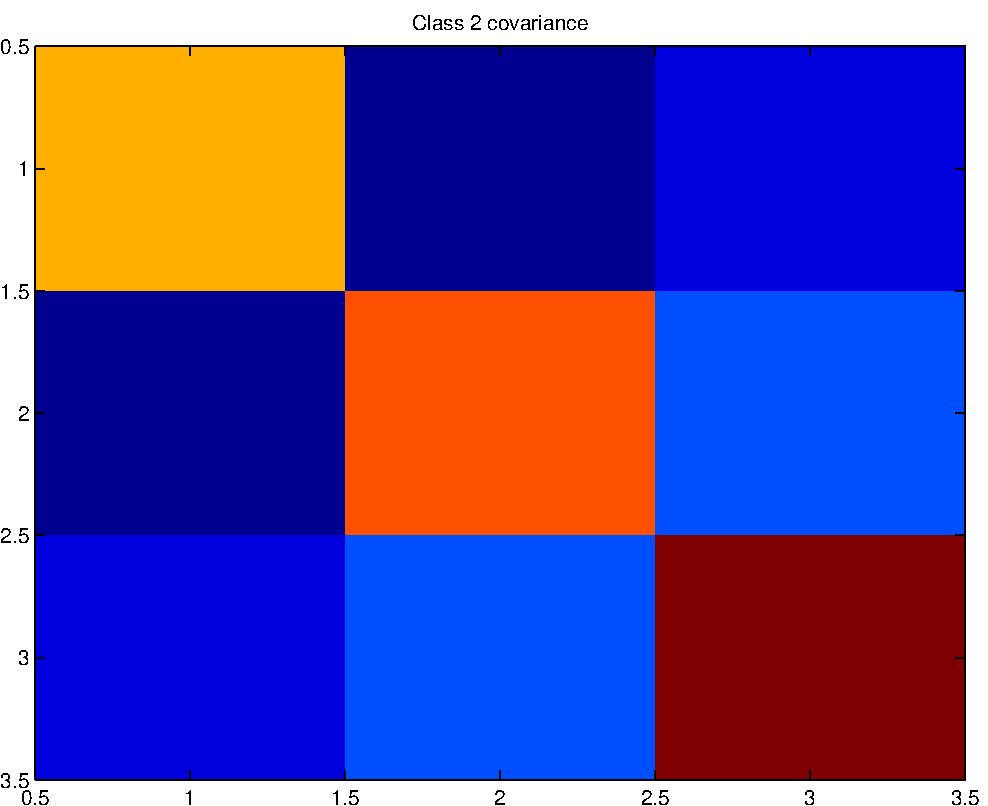
\includegraphics[width=10.0cm,height=10.0cm]{rv2_corr.pdf}

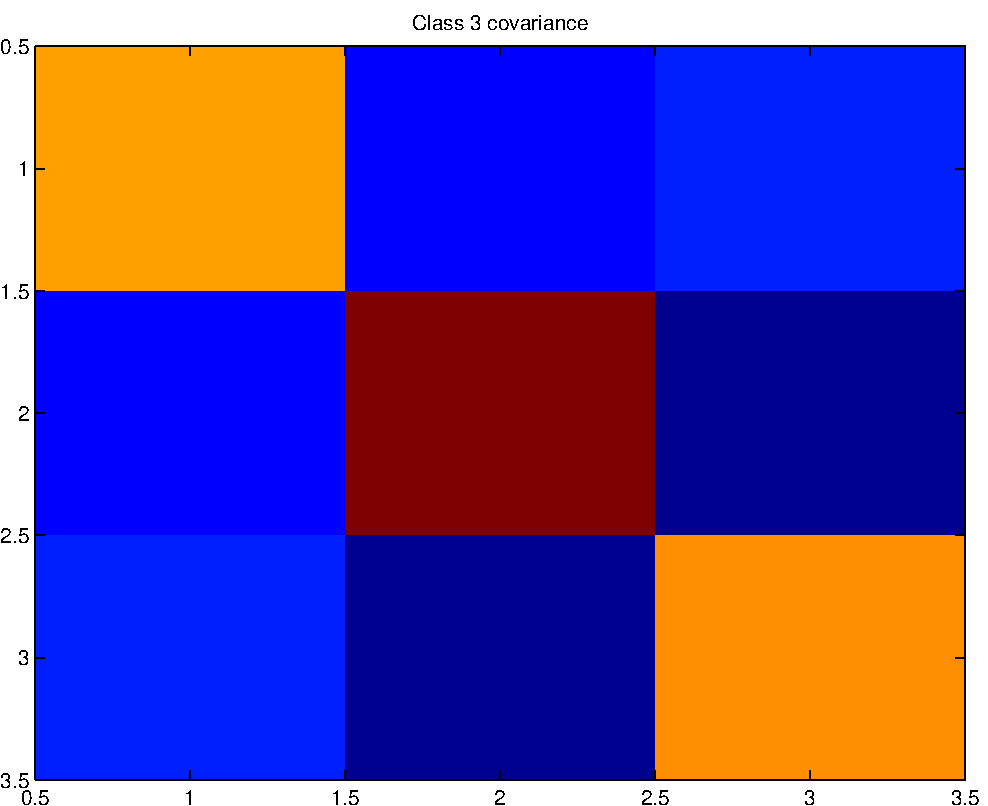
\includegraphics[width=10.0cm,height=10.0cm]{rv3_corr.pdf}

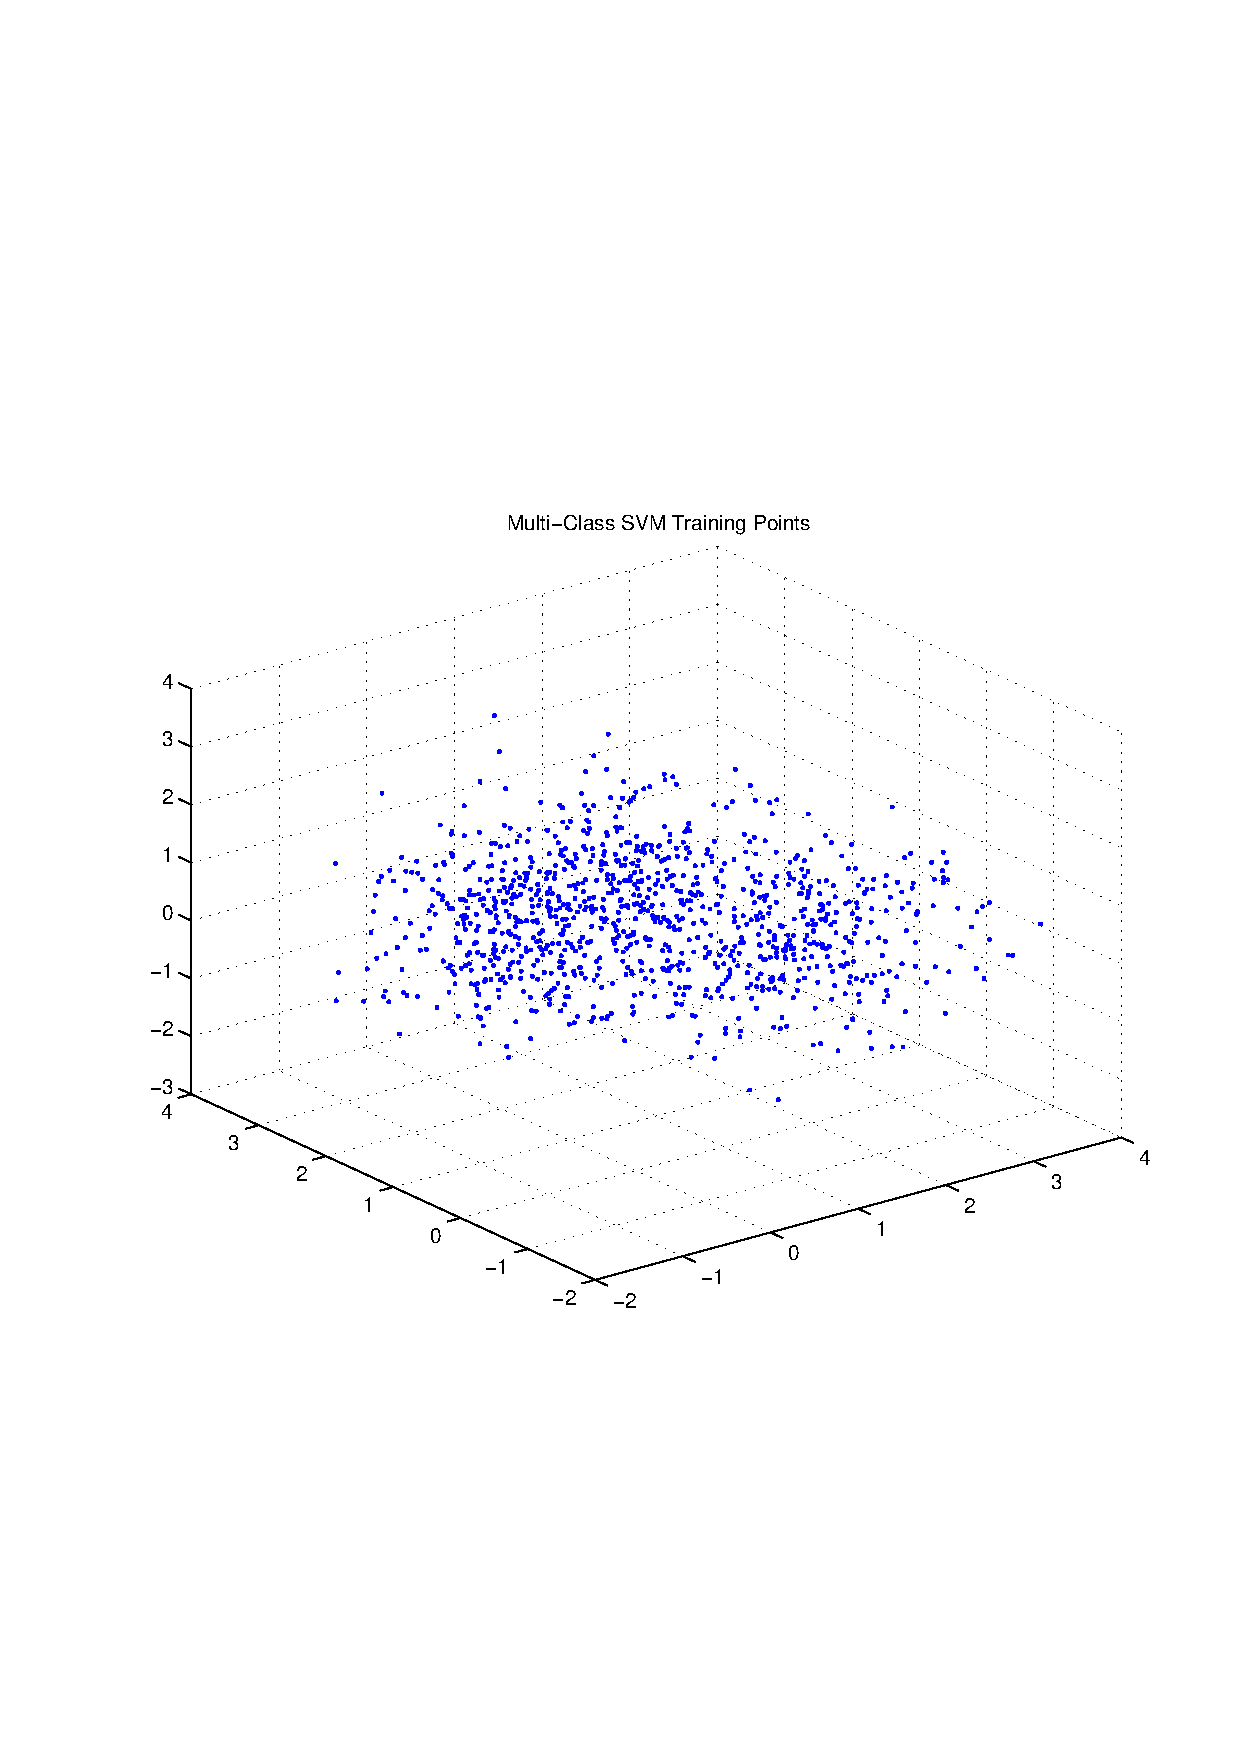
\includegraphics[width=10.0cm,height=10.0cm]{trainingPoints.pdf}

These are the SVM parameters - the RBF kernel is used\begin{itemize}
\item allOutlierFraction=0.05
\item mixingCoeff=0.3
\item smoThresh=1.0/10000.0
\item sigma=1
\end{itemize}
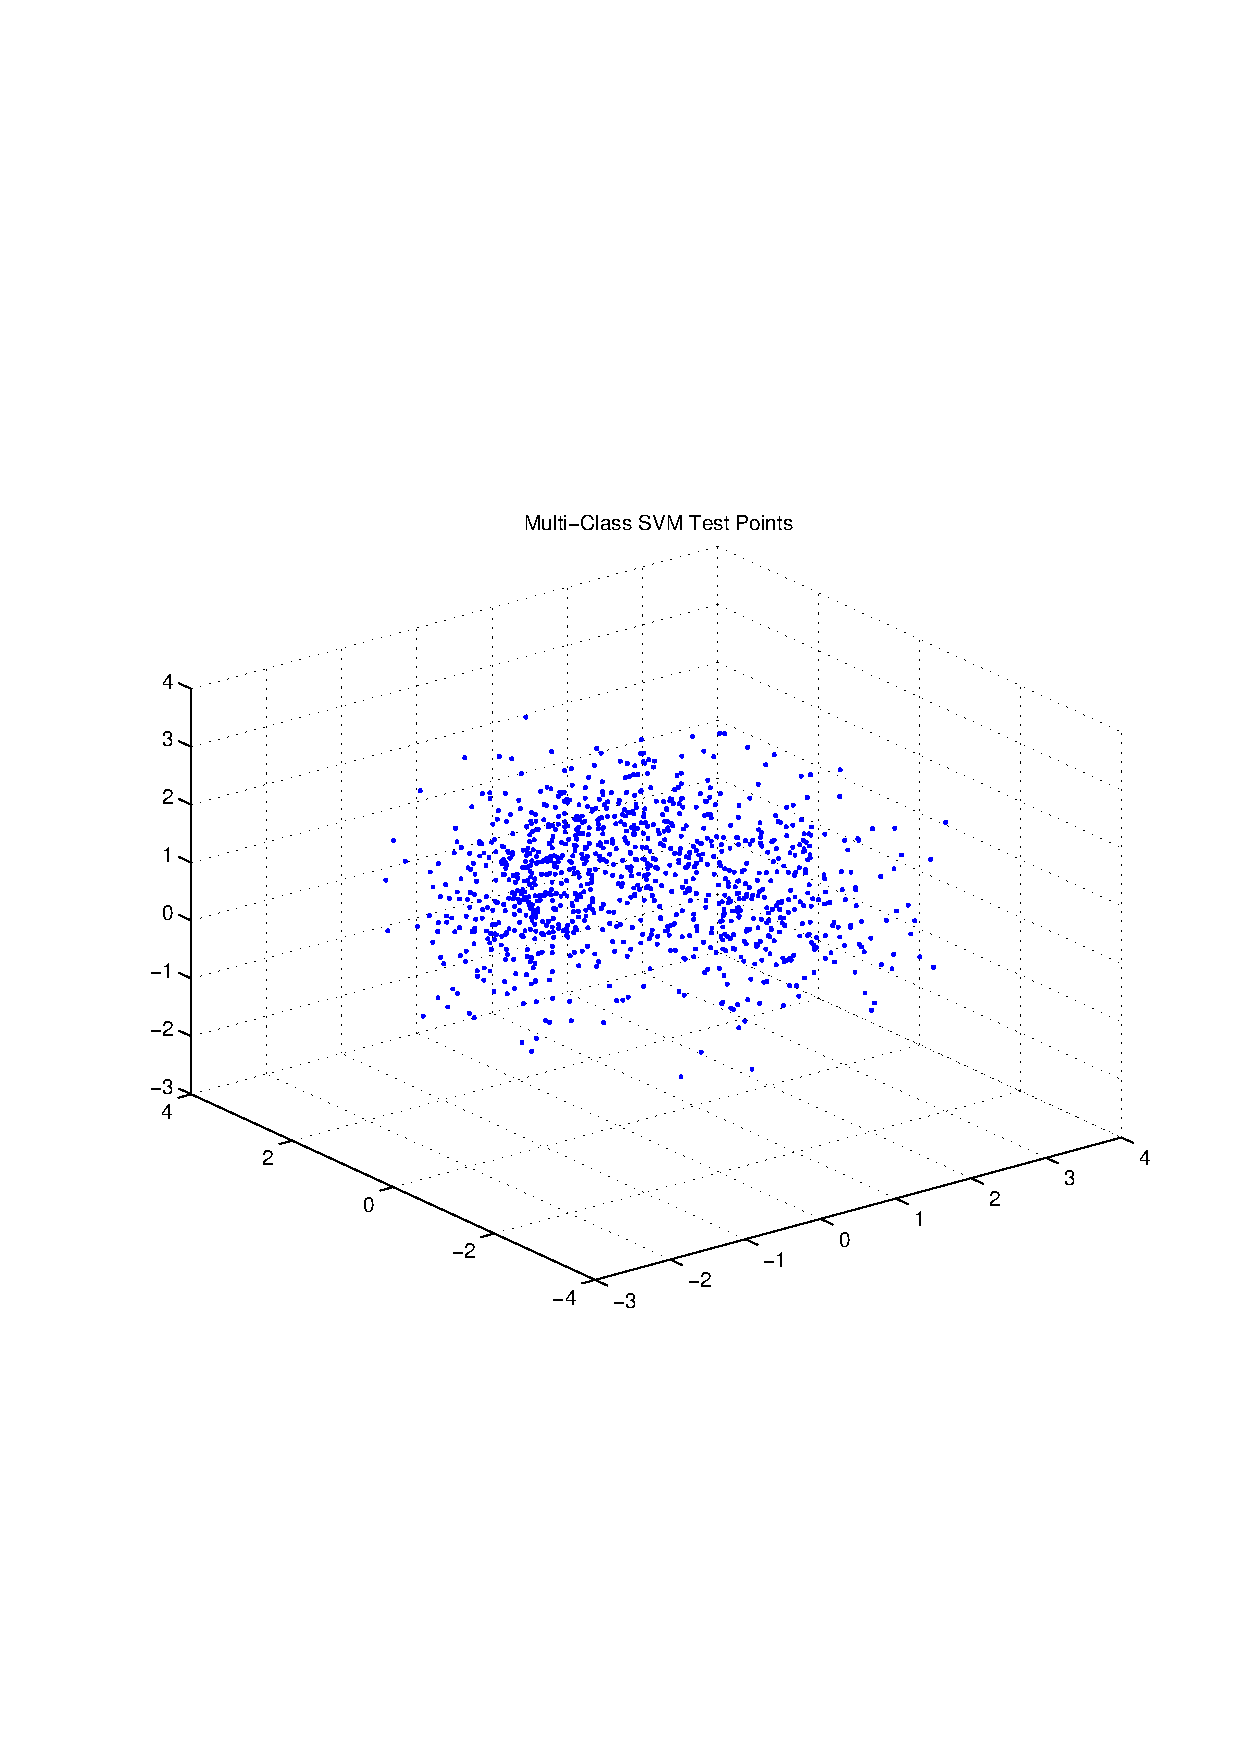
\includegraphics[width=10.0cm,height=10.0cm]{testPoints.pdf}

The marginal sample moments (mean var skew kurtosis) for training points.\newline
\begin{tabular}{ c |  c  c  c  c}
Feature & $\mu_1$ & $\mu_2$ & $\mu_3$ & $\mu_4$ \\
0 & +0.667 & +1.350 & -0.014& +2.184 \\
\hline
1 & +0.702 & +1.264 & +0.051& +2.095 \\
\hline
2 & +0.707 & +1.182 & +0.438& +2.425 \\
\hline
\end{tabular}
\newline
The marginal sample moments (mean var skew kurtosis) for test points.\newline
\begin{tabular}{ c | c  c  c  c}
Feature & $\mu_1$ & $\mu_2$ & $\mu_3$ & $\mu_4$ \\
0 & +0.676 & +1.237 & +0.126& +2.168\\
\hline
1 & +0.664 & +1.271 & +0.098& +2.113\\
\hline
2 & +0.724 & +1.120 & +0.421& +2.343\\
\hline
\end{tabular}\newline
\includegraphics[width=10.0cm,height=10.0cm]{classDiffs.pdf}

The error rate for this run is +0.124\newline
QueryPerformanceCounter  =  +11.024
\subsubsection{Multiclass Support Vector Machine }
\begin{itemize}
\item Number or training points = 1024
\item Feature dimension = 3
\item Number or classes = 3
\end{itemize}
{The mean vectors of the 3 classes}

$\mu_1 = \left(
\begin{array}{
ccc}
+1.90000 & +0.10000 & +0.10000 \\
\end{array}
\right)$

$\mu_2 = \left(
\begin{array}{
ccc}
+0.10000 & +1.90000 & +0.10000 \\
\end{array}
\right)$

$\mu_3 = \left(
\begin{array}{
ccc}
+0.00000 & +0.00000 & +1.90000 \\
\end{array}
\right)$

A random SPD covairance matrix is generated for each of the classes.\newline

$\rho_1 = \left(
\begin{array}{
ccc}
+1.842 & +0.052 & +0.135 \\
+0.052 & +3.713 & +0.435 \\
+0.135 & +0.435 & +3.208 \\
\end{array}
\right)$

$\rho_2 = \left(
\begin{array}{
ccc}
+4.446 & +0.177 & -0.354 \\
+0.177 & +1.548 & -0.441 \\
-0.354 & -0.441 & +2.538 \\
\end{array}
\right)$

$\rho_3 = \left(
\begin{array}{
ccc}
+1.709 & +0.120 & -0.370 \\
+0.120 & +2.197 & +0.042 \\
-0.370 & +0.042 & +1.933 \\
\end{array}
\right)$

Verify $L_1$ condition number of covariance. The diagonal entries of the matrix have the form $(0.5 + U(0,1) )*dim(Dom(Cov))$
The lower-diagonal entries take the form $U(0,1) - 0.5$. 
The $L_1$ condition numbers are :
\begin{itemize}
\item +2.402
\item +4.055
\item +1.810
\end{itemize}
\includegraphics[width=10.0cm,height=10.0cm]{rv1_corr.pdf}

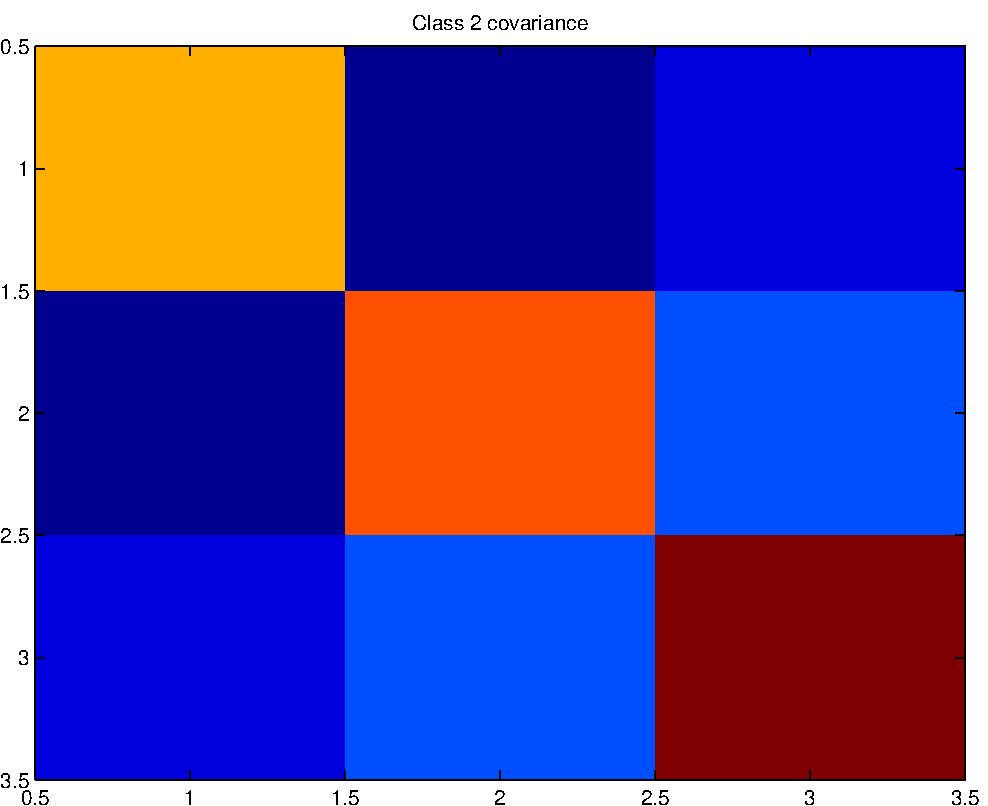
\includegraphics[width=10.0cm,height=10.0cm]{rv2_corr.pdf}

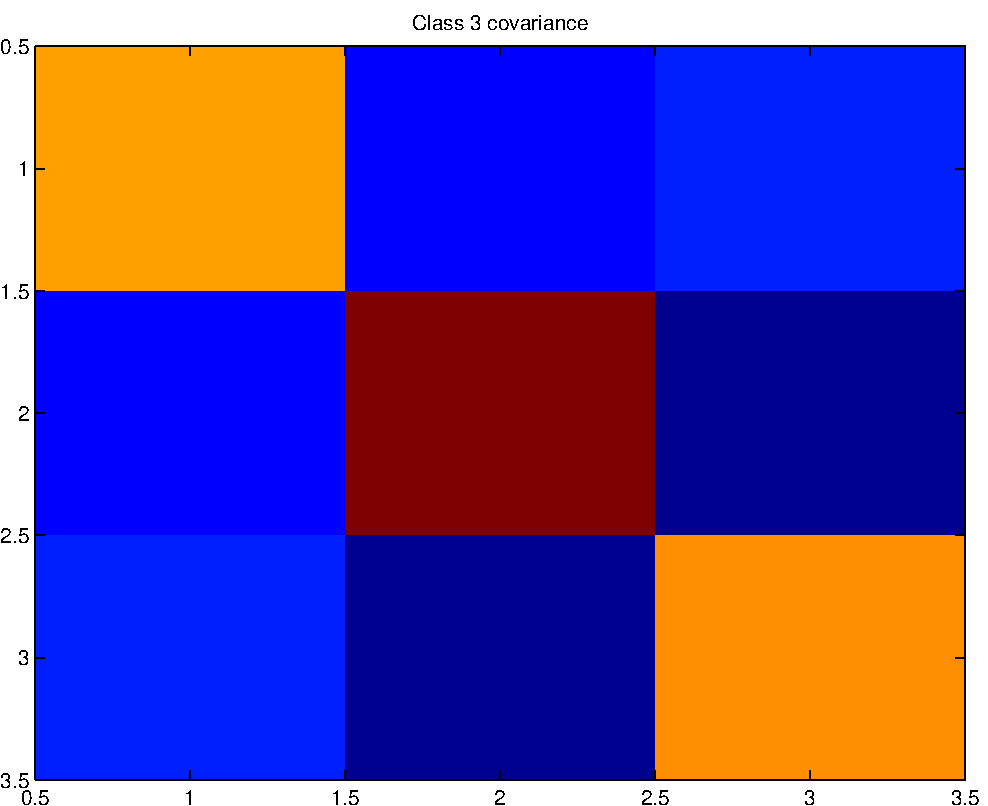
\includegraphics[width=10.0cm,height=10.0cm]{rv3_corr.pdf}

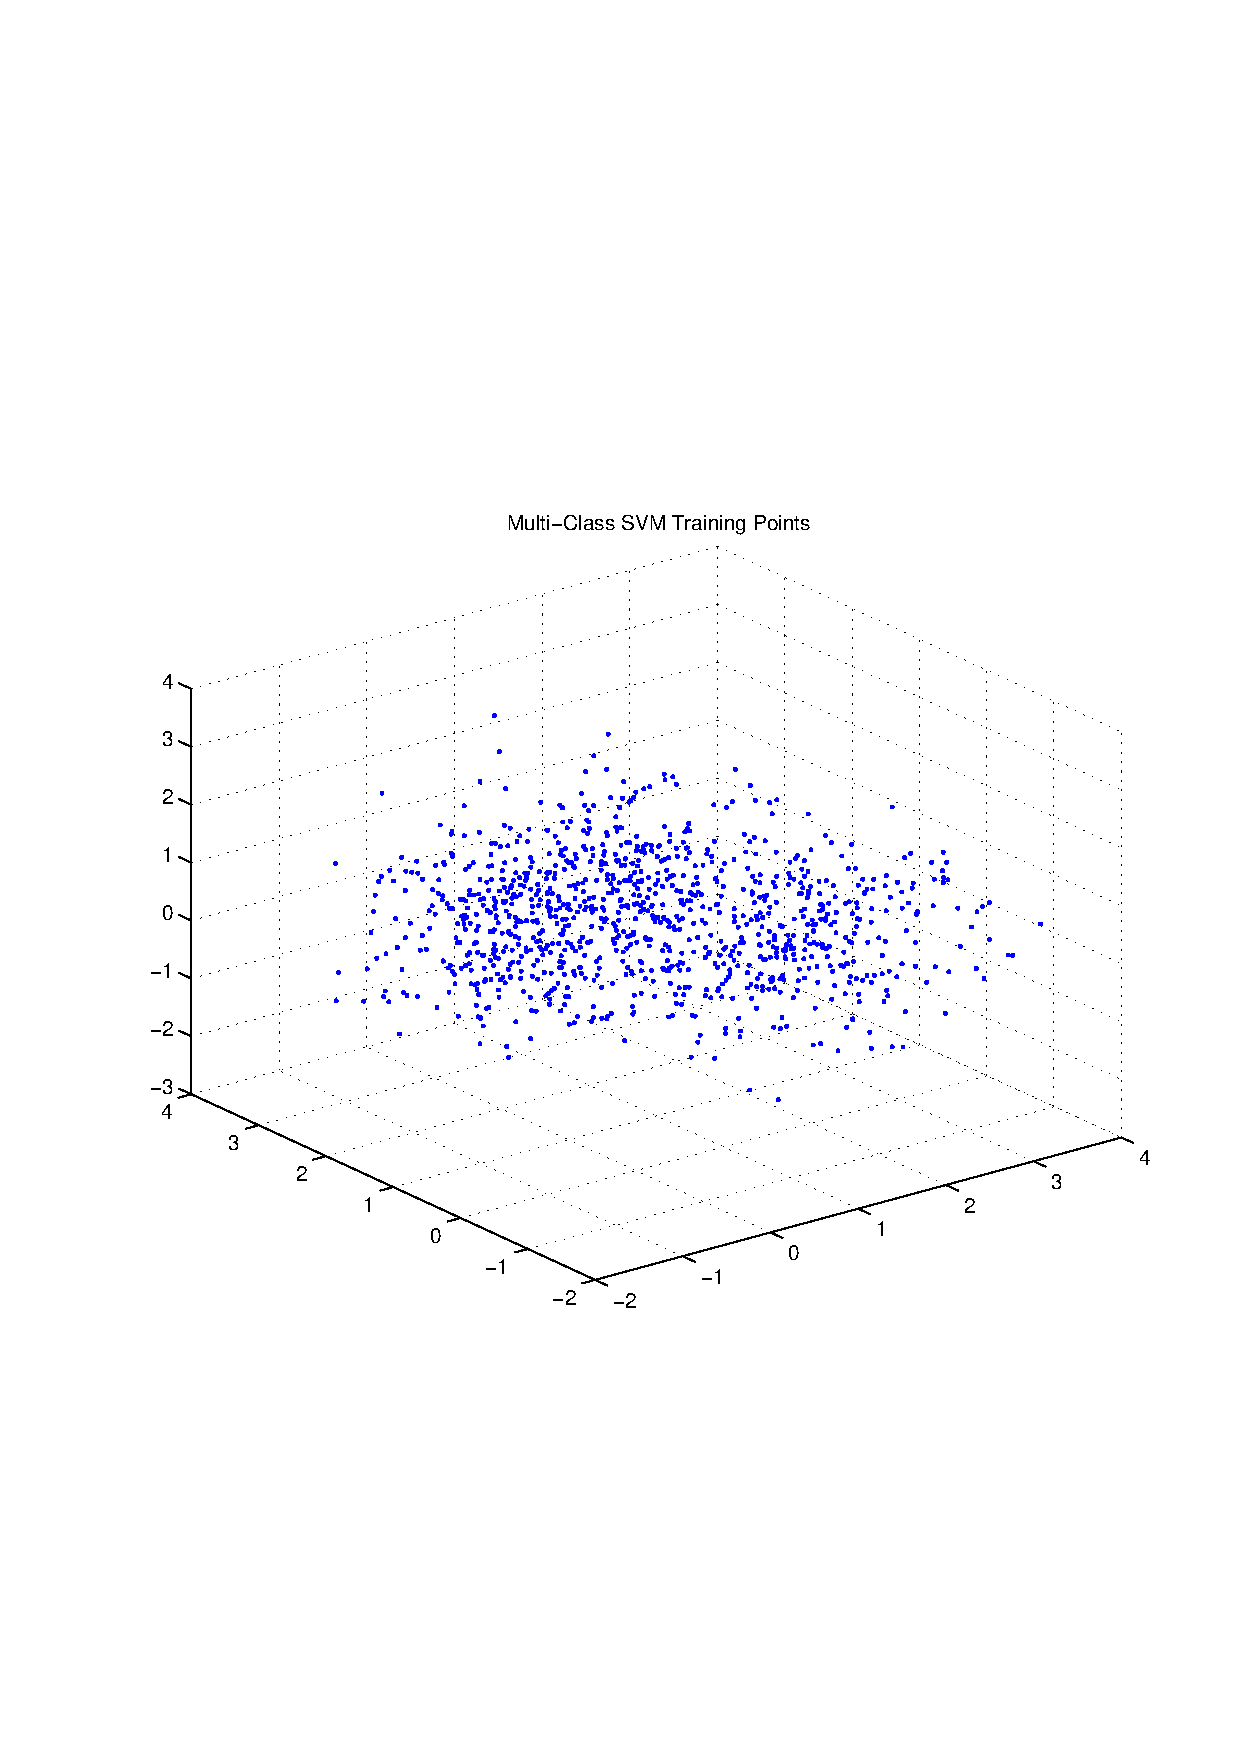
\includegraphics[width=10.0cm,height=10.0cm]{trainingPoints.pdf}

These are the SVM parameters - the RBF kernel is used\begin{itemize}
\item allOutlierFraction=0.05
\item mixingCoeff=0.3
\item smoThresh=1.0/10000.0
\item sigma=1
\end{itemize}
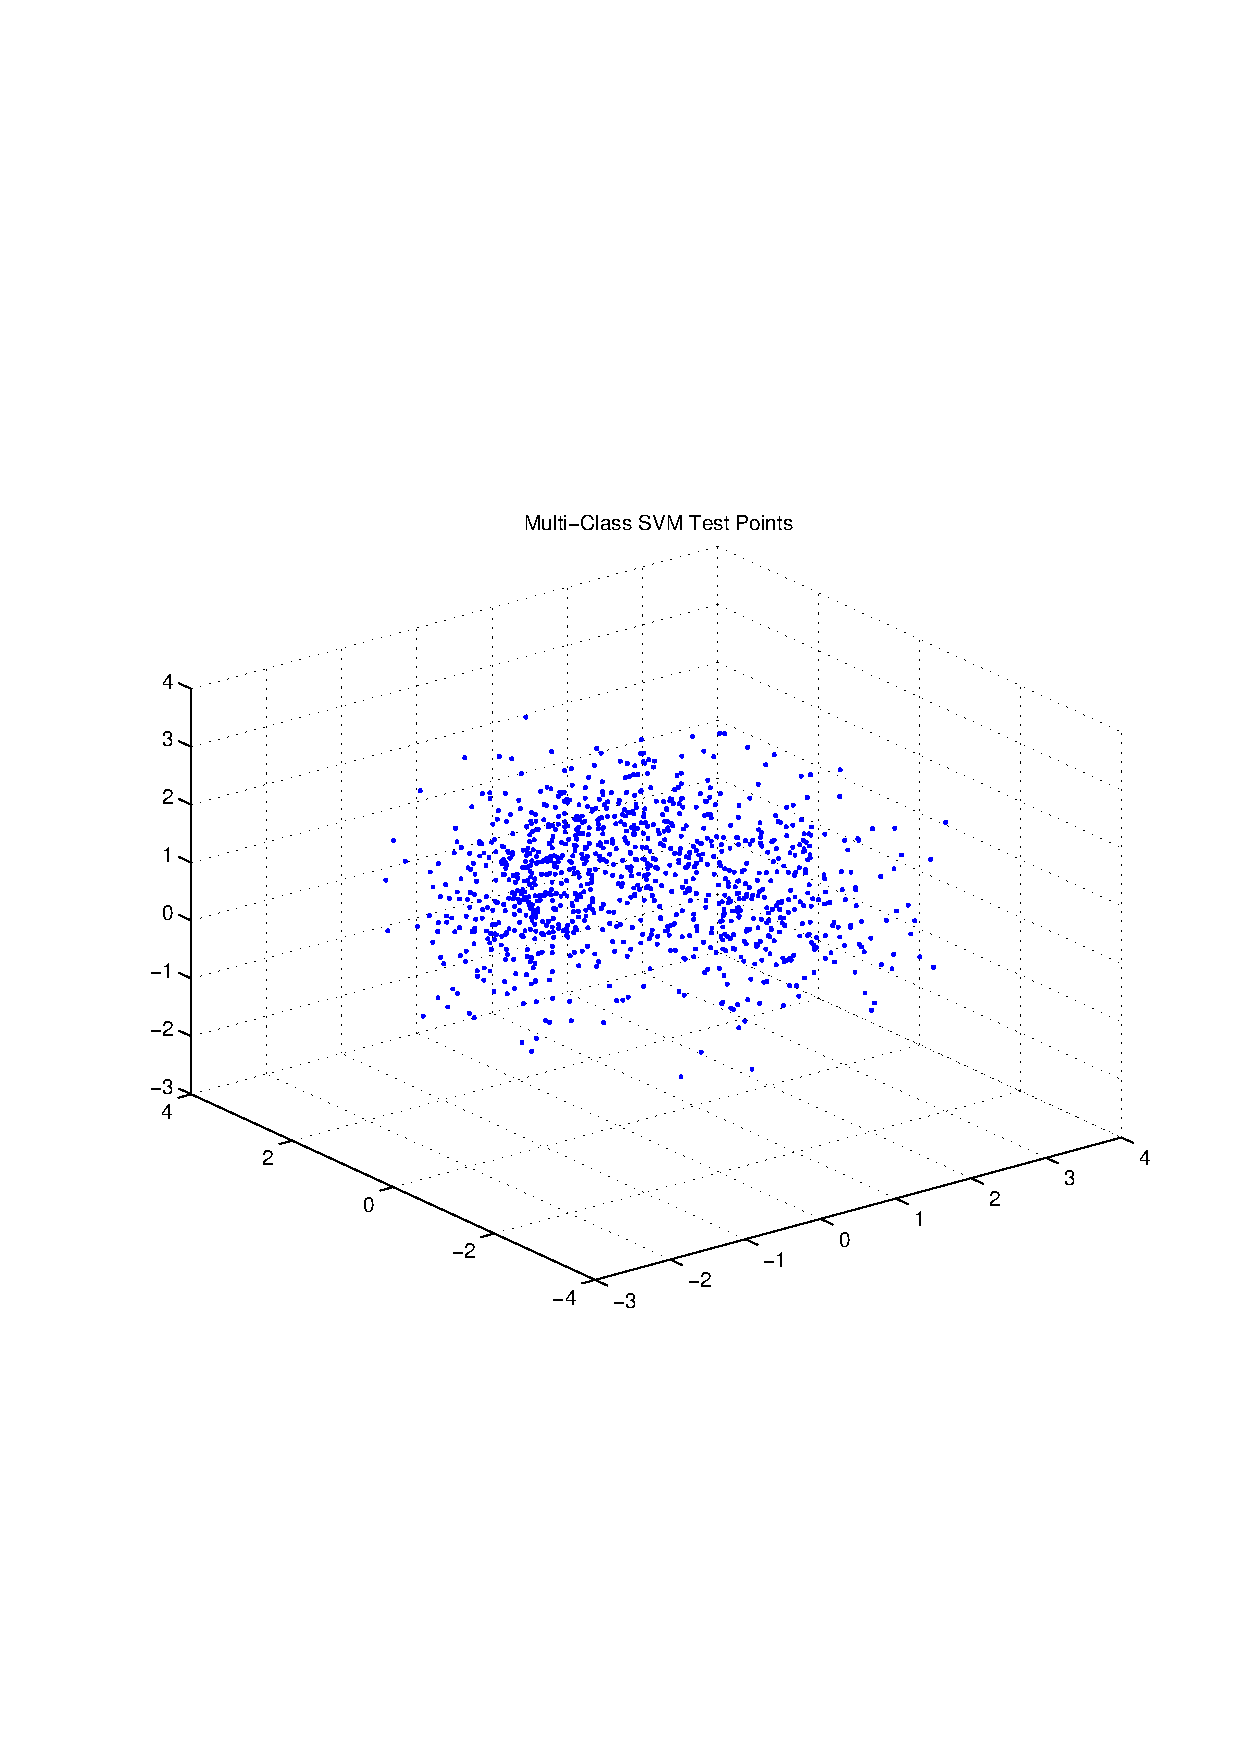
\includegraphics[width=10.0cm,height=10.0cm]{testPoints.pdf}

The marginal sample moments (mean var skew kurtosis) for training points.\newline
\begin{tabular}{ c |  c  c  c  c}
Feature & $\mu_1$ & $\mu_2$ & $\mu_3$ & $\mu_4$ \\
0 & +0.668 & +1.303 & +0.083& +2.263 \\
\hline
1 & +0.699 & +1.189 & +0.142& +2.094 \\
\hline
2 & +0.699 & +1.227 & +0.188& +2.236 \\
\hline
\end{tabular}
\newline
The marginal sample moments (mean var skew kurtosis) for test points.\newline
\begin{tabular}{ c | c  c  c  c}
Feature & $\mu_1$ & $\mu_2$ & $\mu_3$ & $\mu_4$ \\
0 & +0.677 & +1.193 & +0.252& +2.183\\
\hline
1 & +0.665 & +1.194 & +0.191& +2.085\\
\hline
2 & +0.718 & +1.162 & +0.202& +2.149\\
\hline
\end{tabular}\newline
\includegraphics[width=10.0cm,height=10.0cm]{classDiffs.pdf}

The error rate for this run is +0.037\newline
QueryPerformanceCounter  =  +6.966
\subsubsection{Random Number Generator }
The sample size generated for this run is 100000.

\newpage
uniform \begin{tabular}{|c|c|c|c|}  mean & variance & skewness & kurtosis \\  \hline
$\mu_1 = +0.500$ & $\mu_2 = +0.084$ & $\mu_3 = +0.003$ & $\mu_4 =+1.801$ \\
\end{tabular}

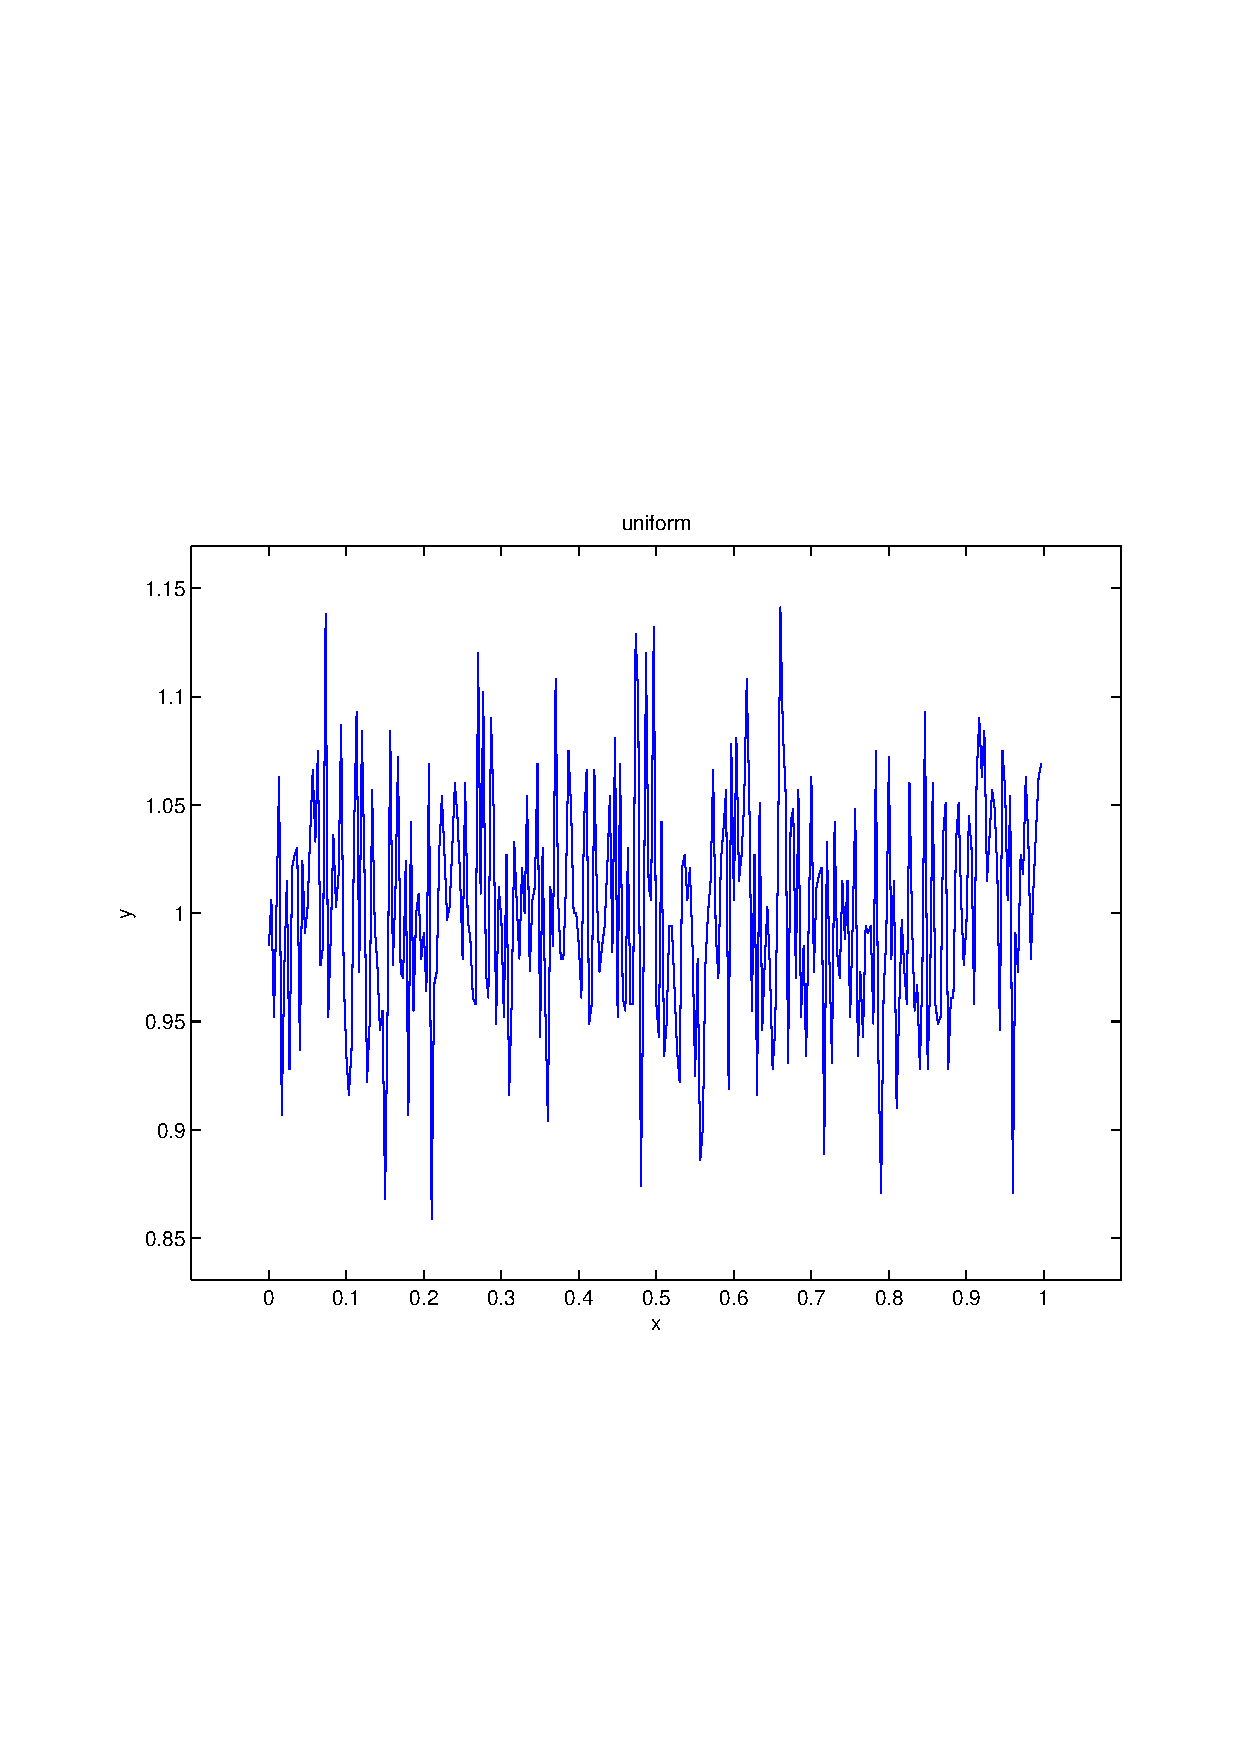
\includegraphics[width=5cm,height=5cm]{uniform.pdf}

cauchy \begin{tabular}{|c|c|c|c|}  mean & variance & skewness & kurtosis \\  \hline
$\mu_1 = +0.443$ & $\mu_2 = +0.053$ & $\mu_3 = +0.639$ & $\mu_4 =+3.281$ \\
\end{tabular}

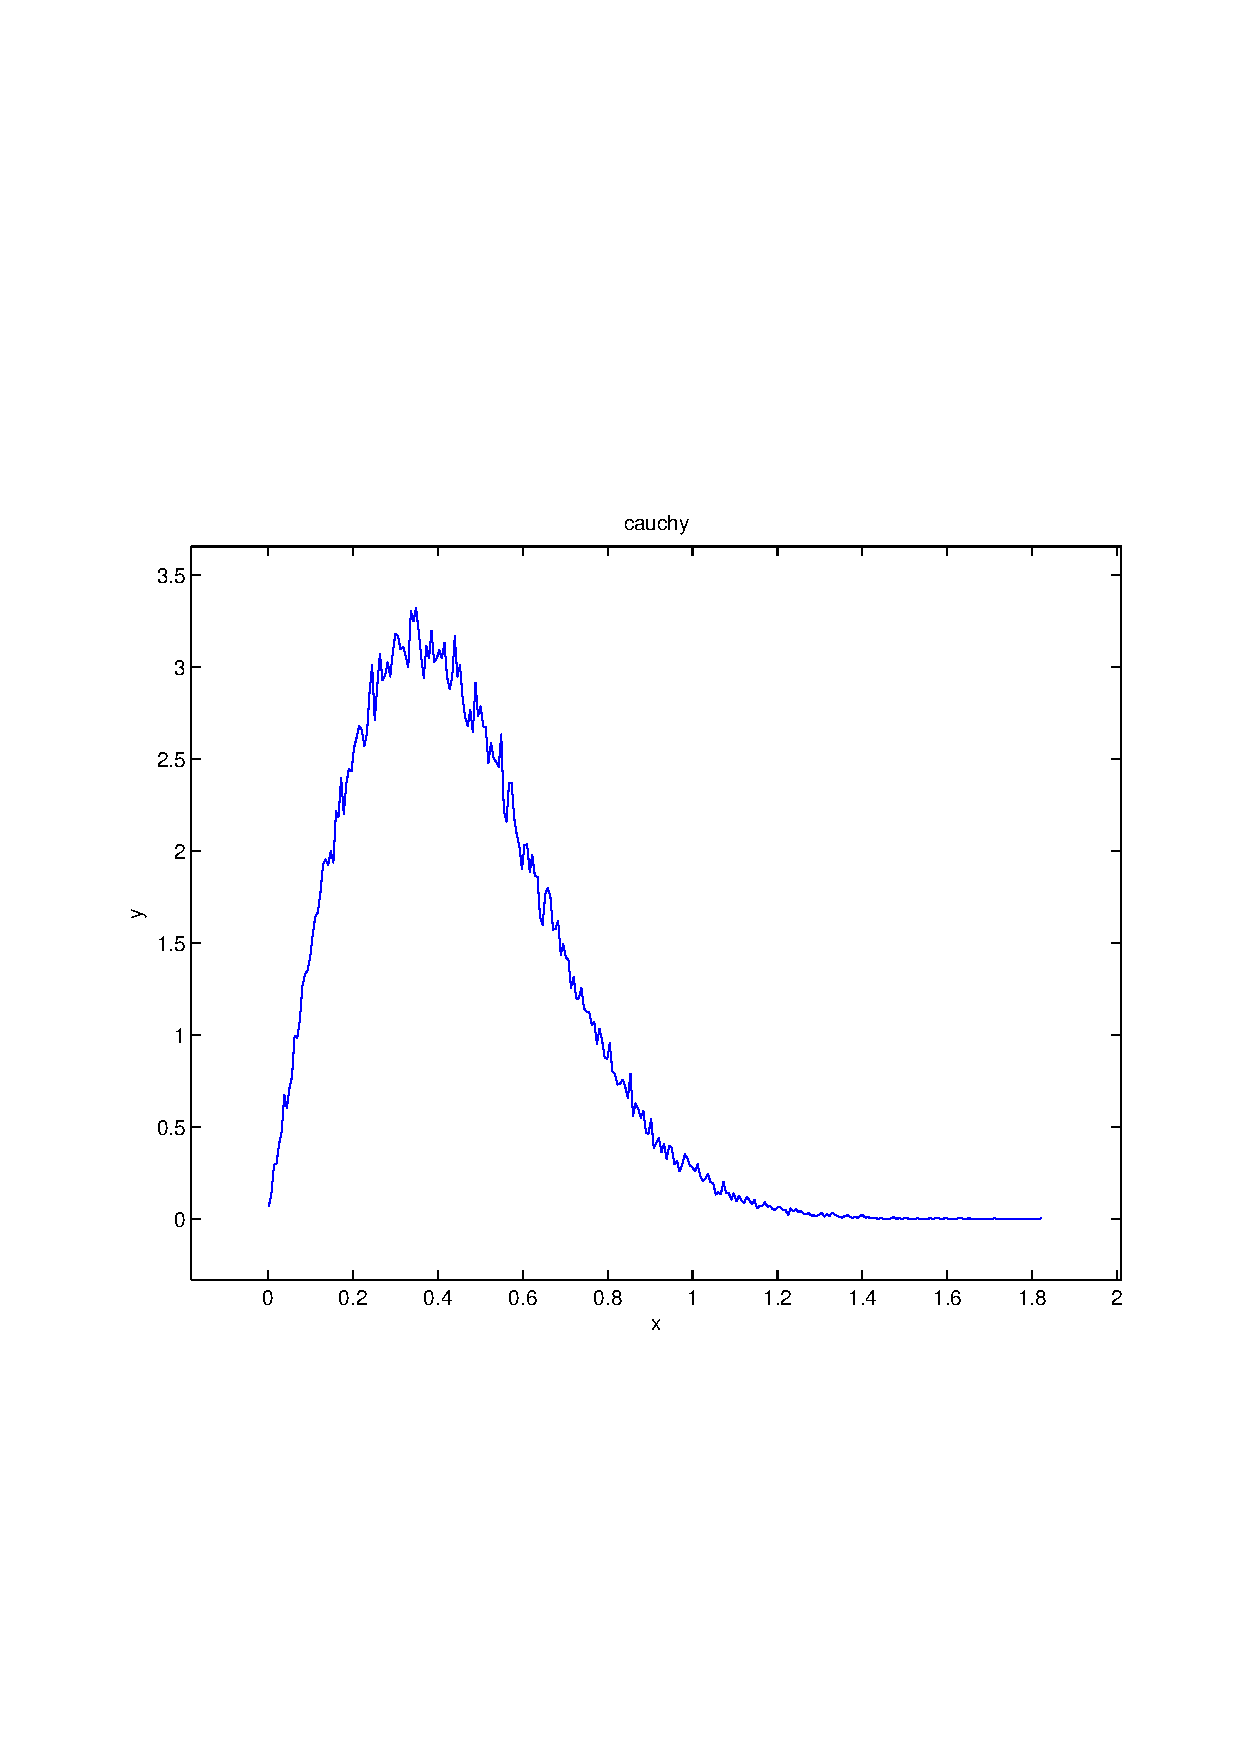
\includegraphics[width=5cm,height=5cm]{cauchy.pdf}

exponential \begin{tabular}{|c|c|c|c|}  mean & variance & skewness & kurtosis \\  \hline
$\mu_1 = +1.996$ & $\mu_2 = +3.993$ & $\mu_3 = +2.031$ & $\mu_4 =+9.308$ \\
\end{tabular}

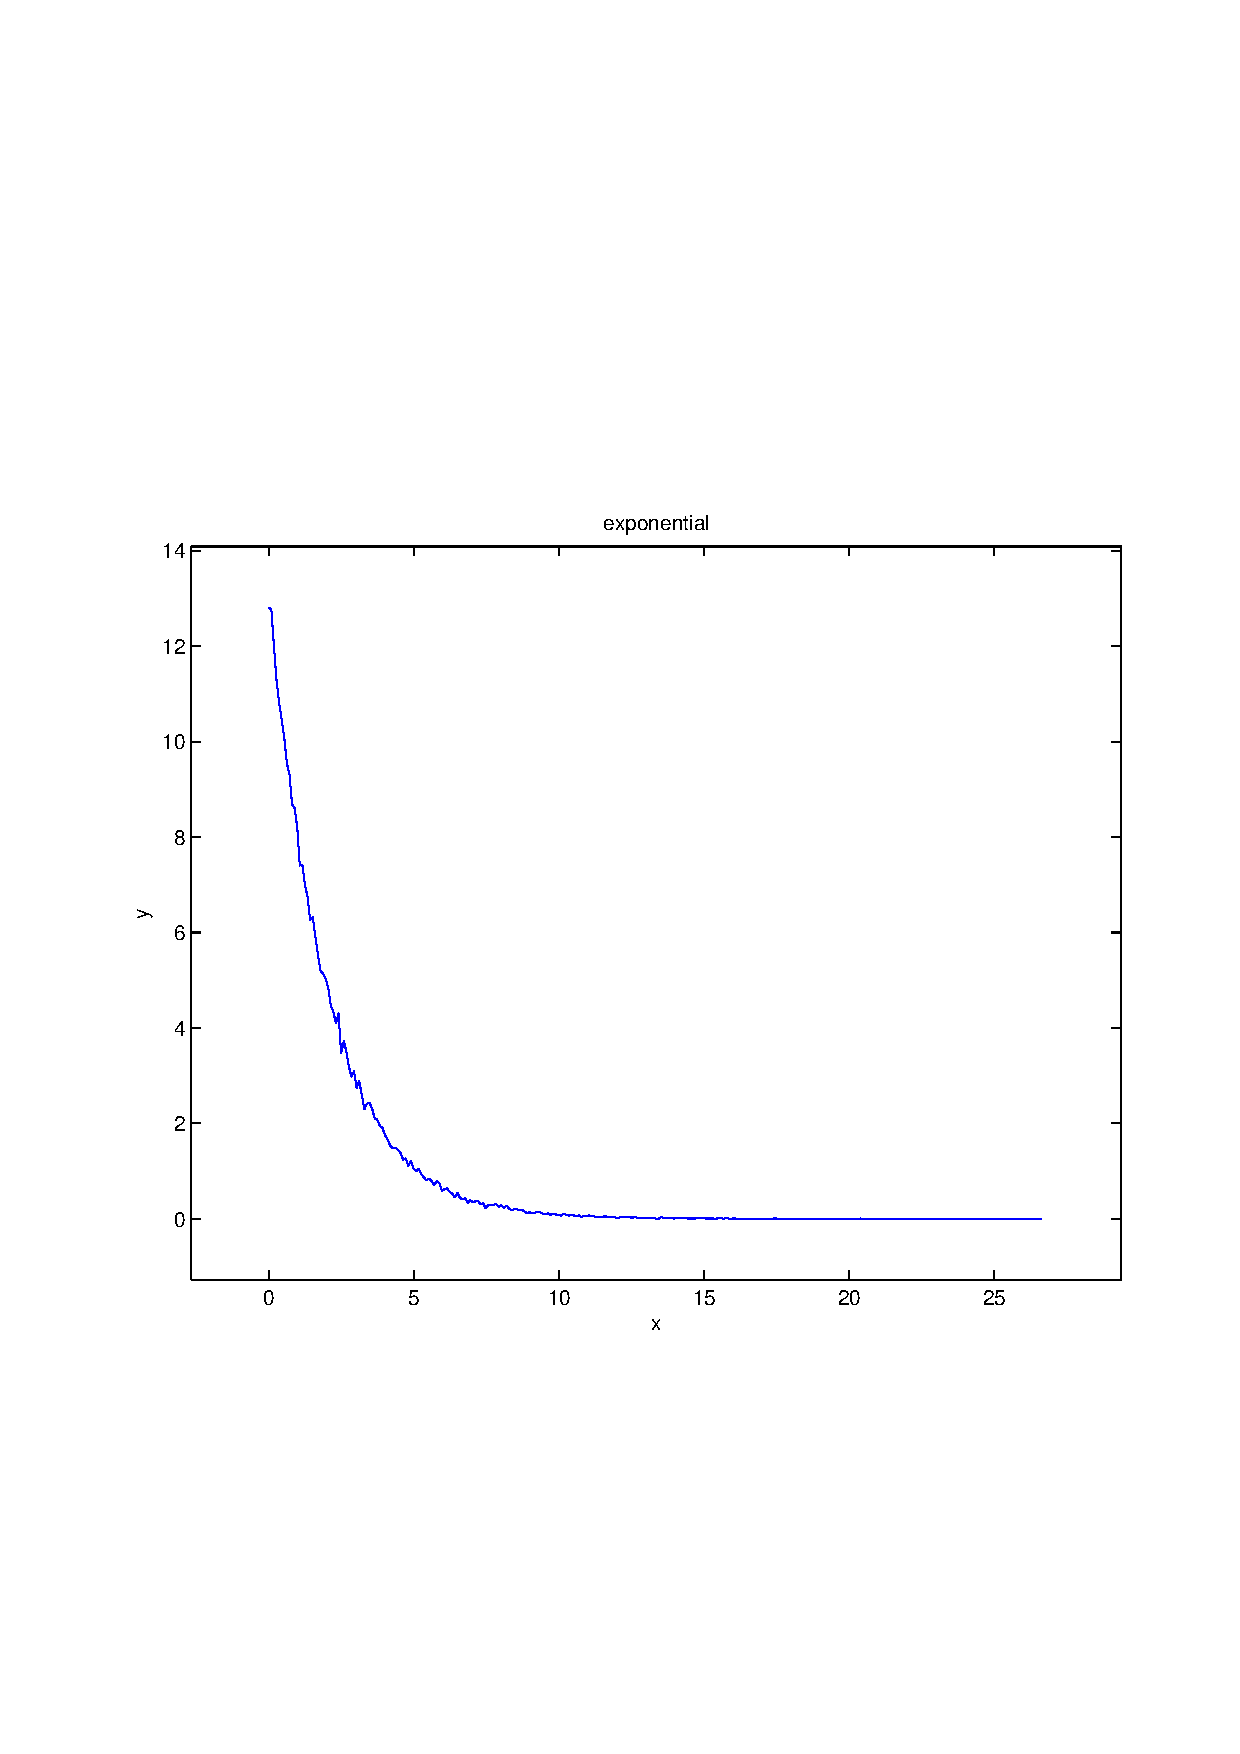
\includegraphics[width=5cm,height=5cm]{exponential.pdf}

\newpage
gamma \begin{tabular}{|c|c|c|c|}  mean & variance & skewness & kurtosis \\  \hline
$\mu_1 = +1.900$ & $\mu_2 = +1.895$ & $\mu_3 = +1.434$ & $\mu_4 =+6.060$ \\
\end{tabular}

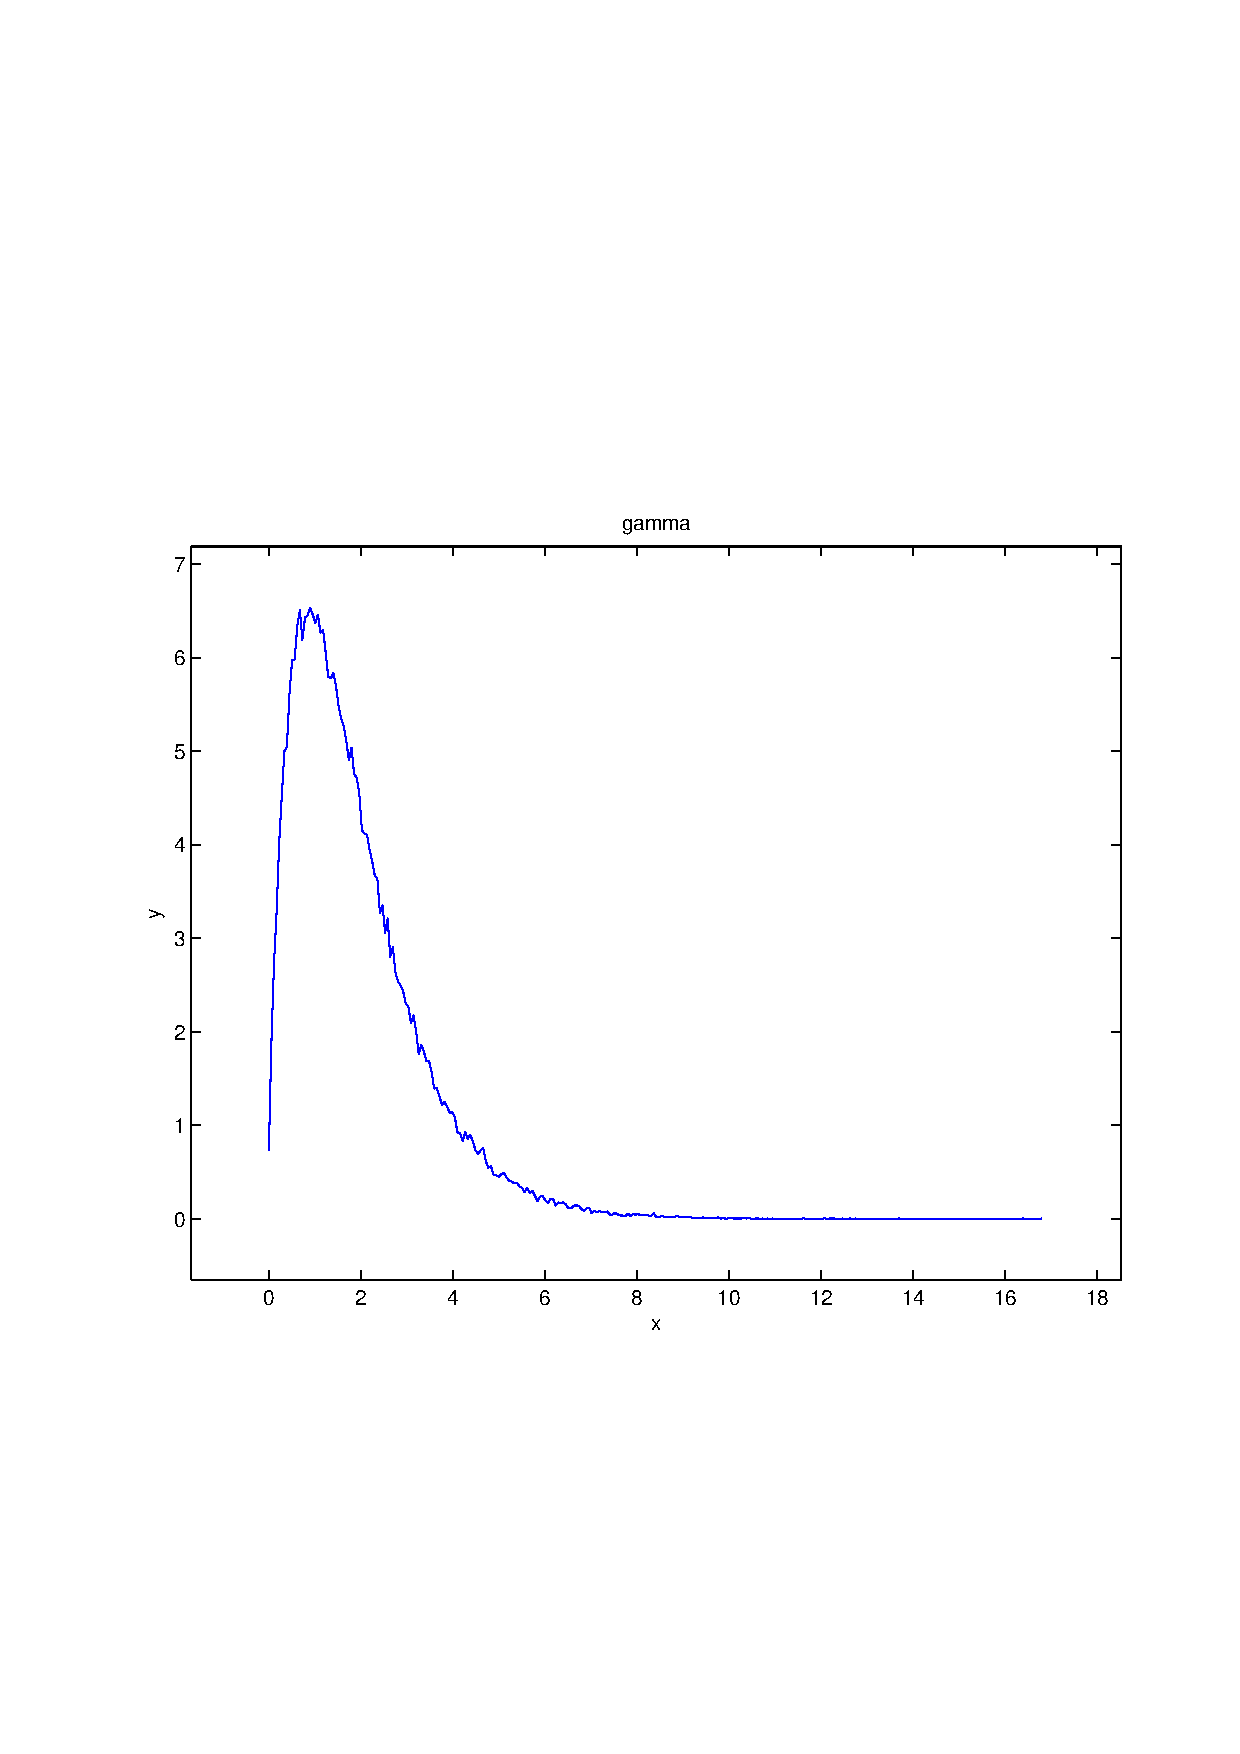
\includegraphics[width=5cm,height=5cm]{gamma.pdf}

GIG \begin{tabular}{|c|c|c|c|}  mean & variance & skewness & kurtosis \\  \hline
$\mu_1 = +0.804$ & $\mu_2 = +11.337$ & $\mu_3 = +15.334$ & $\mu_4 =+308.819$ \\
\end{tabular}

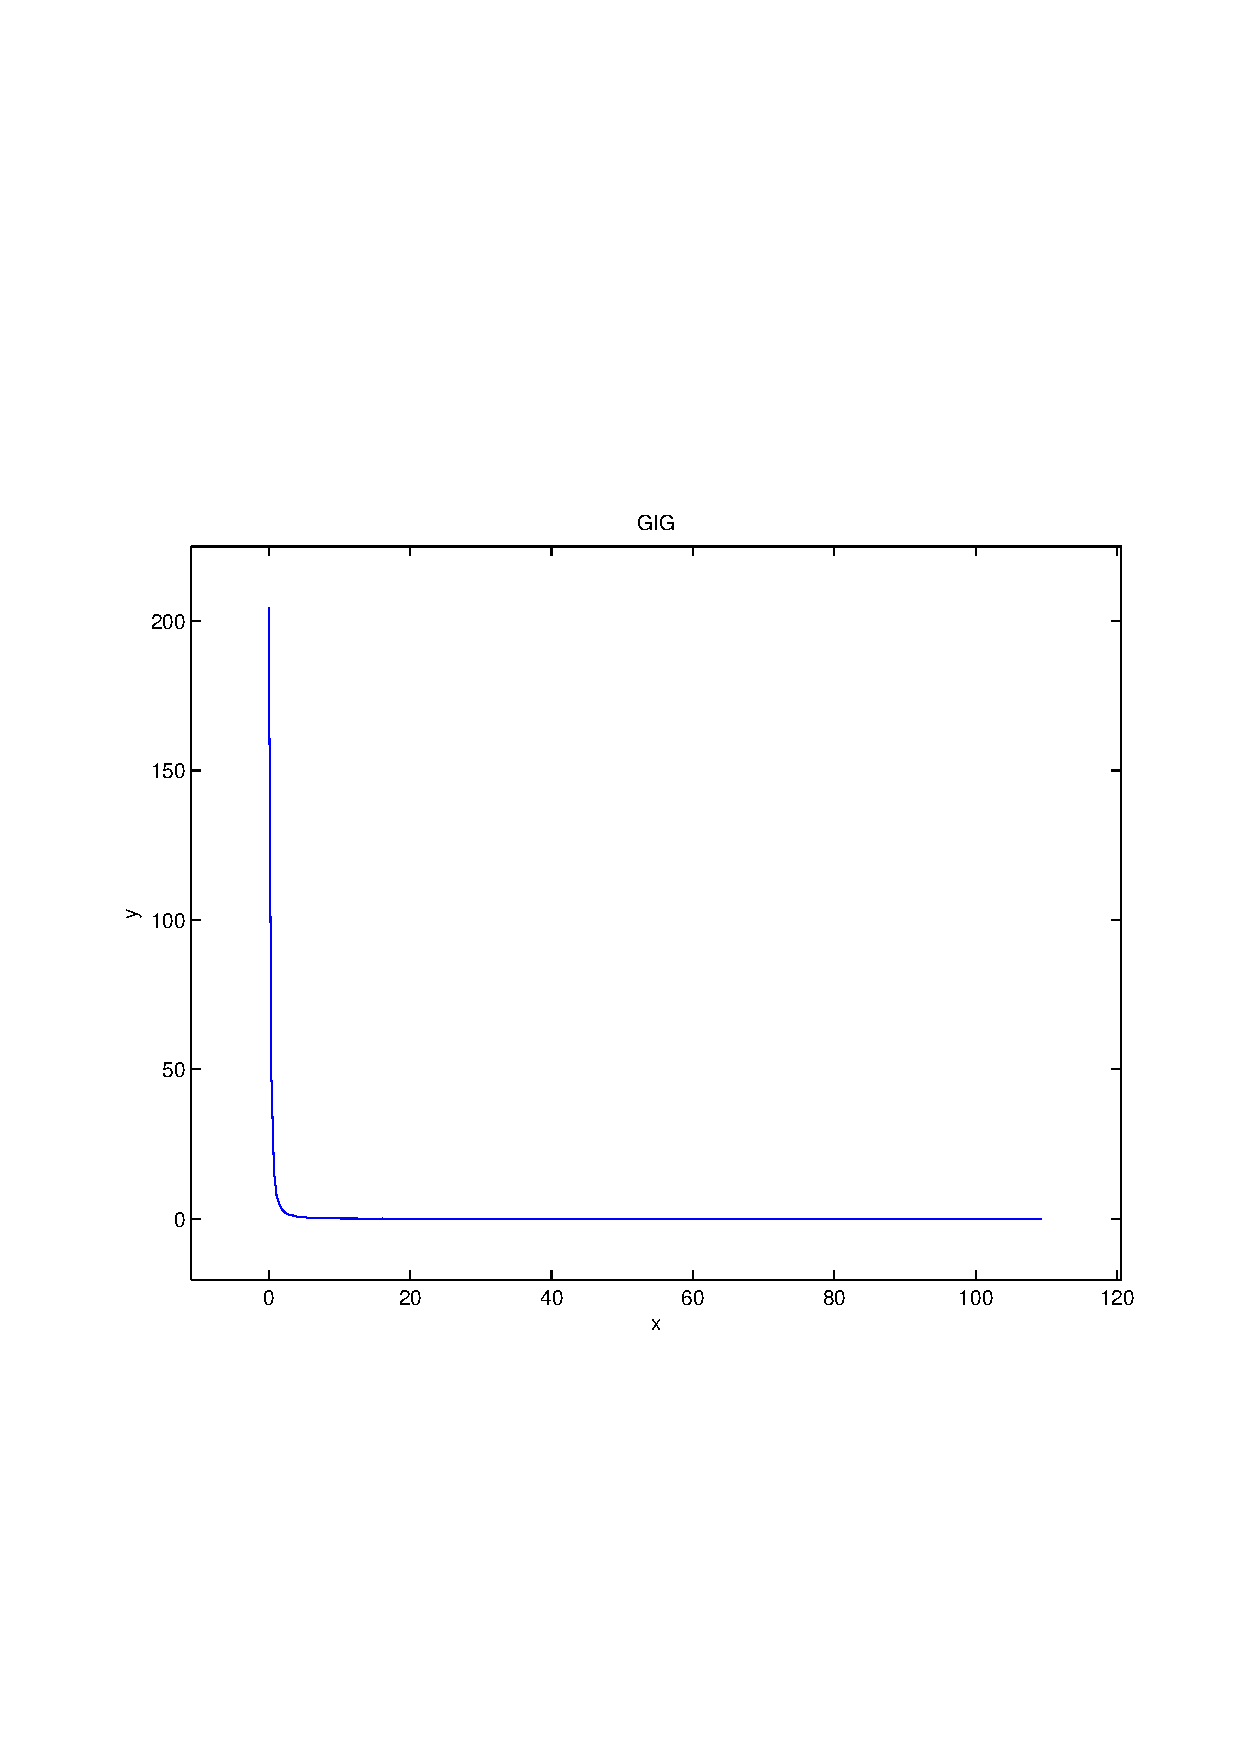
\includegraphics[width=5cm,height=5cm]{GIG.pdf}

normal-box-muller \begin{tabular}{|c|c|c|c|}  mean & variance & skewness & kurtosis \\  \hline
$\mu_1 = +0.004$ & $\mu_2 = +0.998$ & $\mu_3 = +0.002$ & $\mu_4 =+2.989$ \\
\end{tabular}

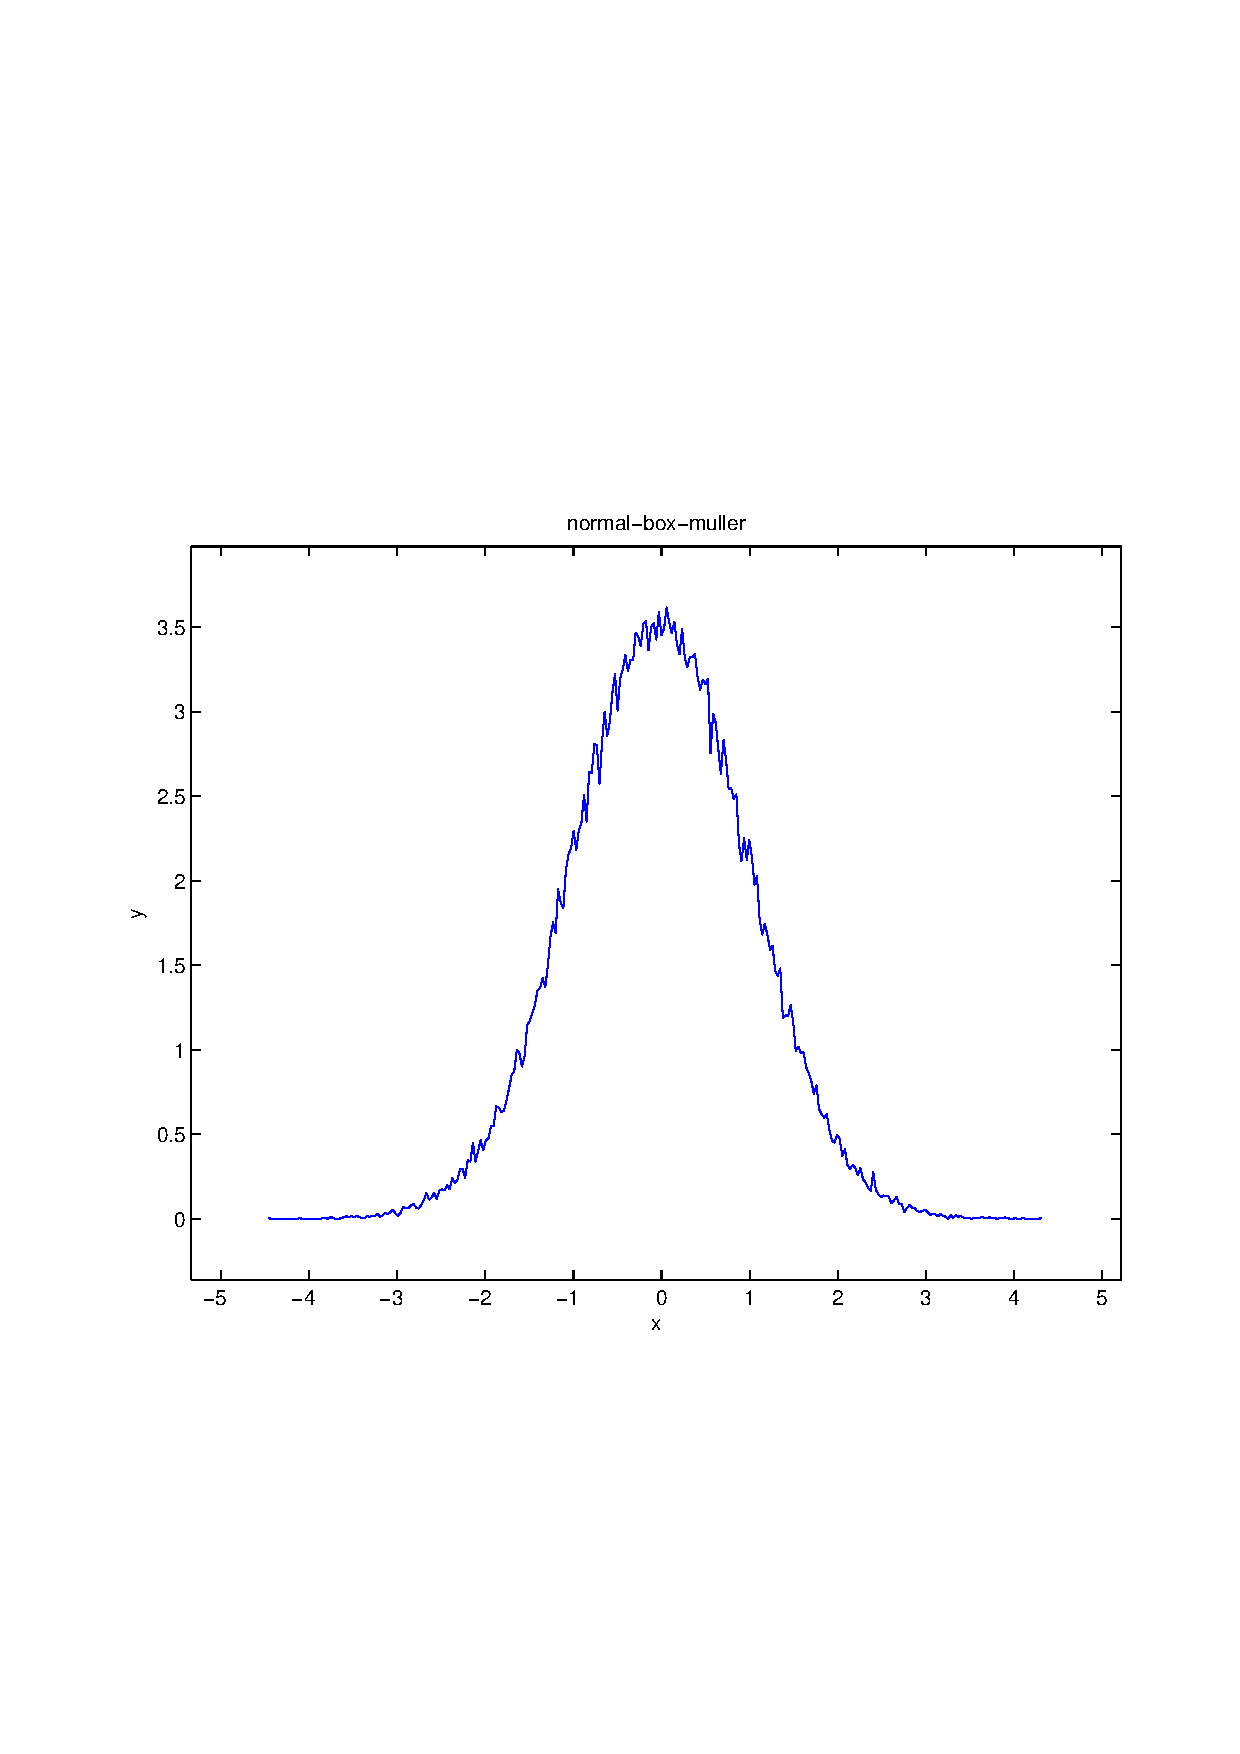
\includegraphics[width=5cm,height=5cm]{normal-box-muller.pdf}

\newpage
normal-inverse-approximation \begin{tabular}{|c|c|c|c|}  mean & variance & skewness & kurtosis \\  \hline
$\mu_1 = +0.002$ & $\mu_2 = +1.005$ & $\mu_3 = +0.012$ & $\mu_4 =+2.993$ \\
\end{tabular}

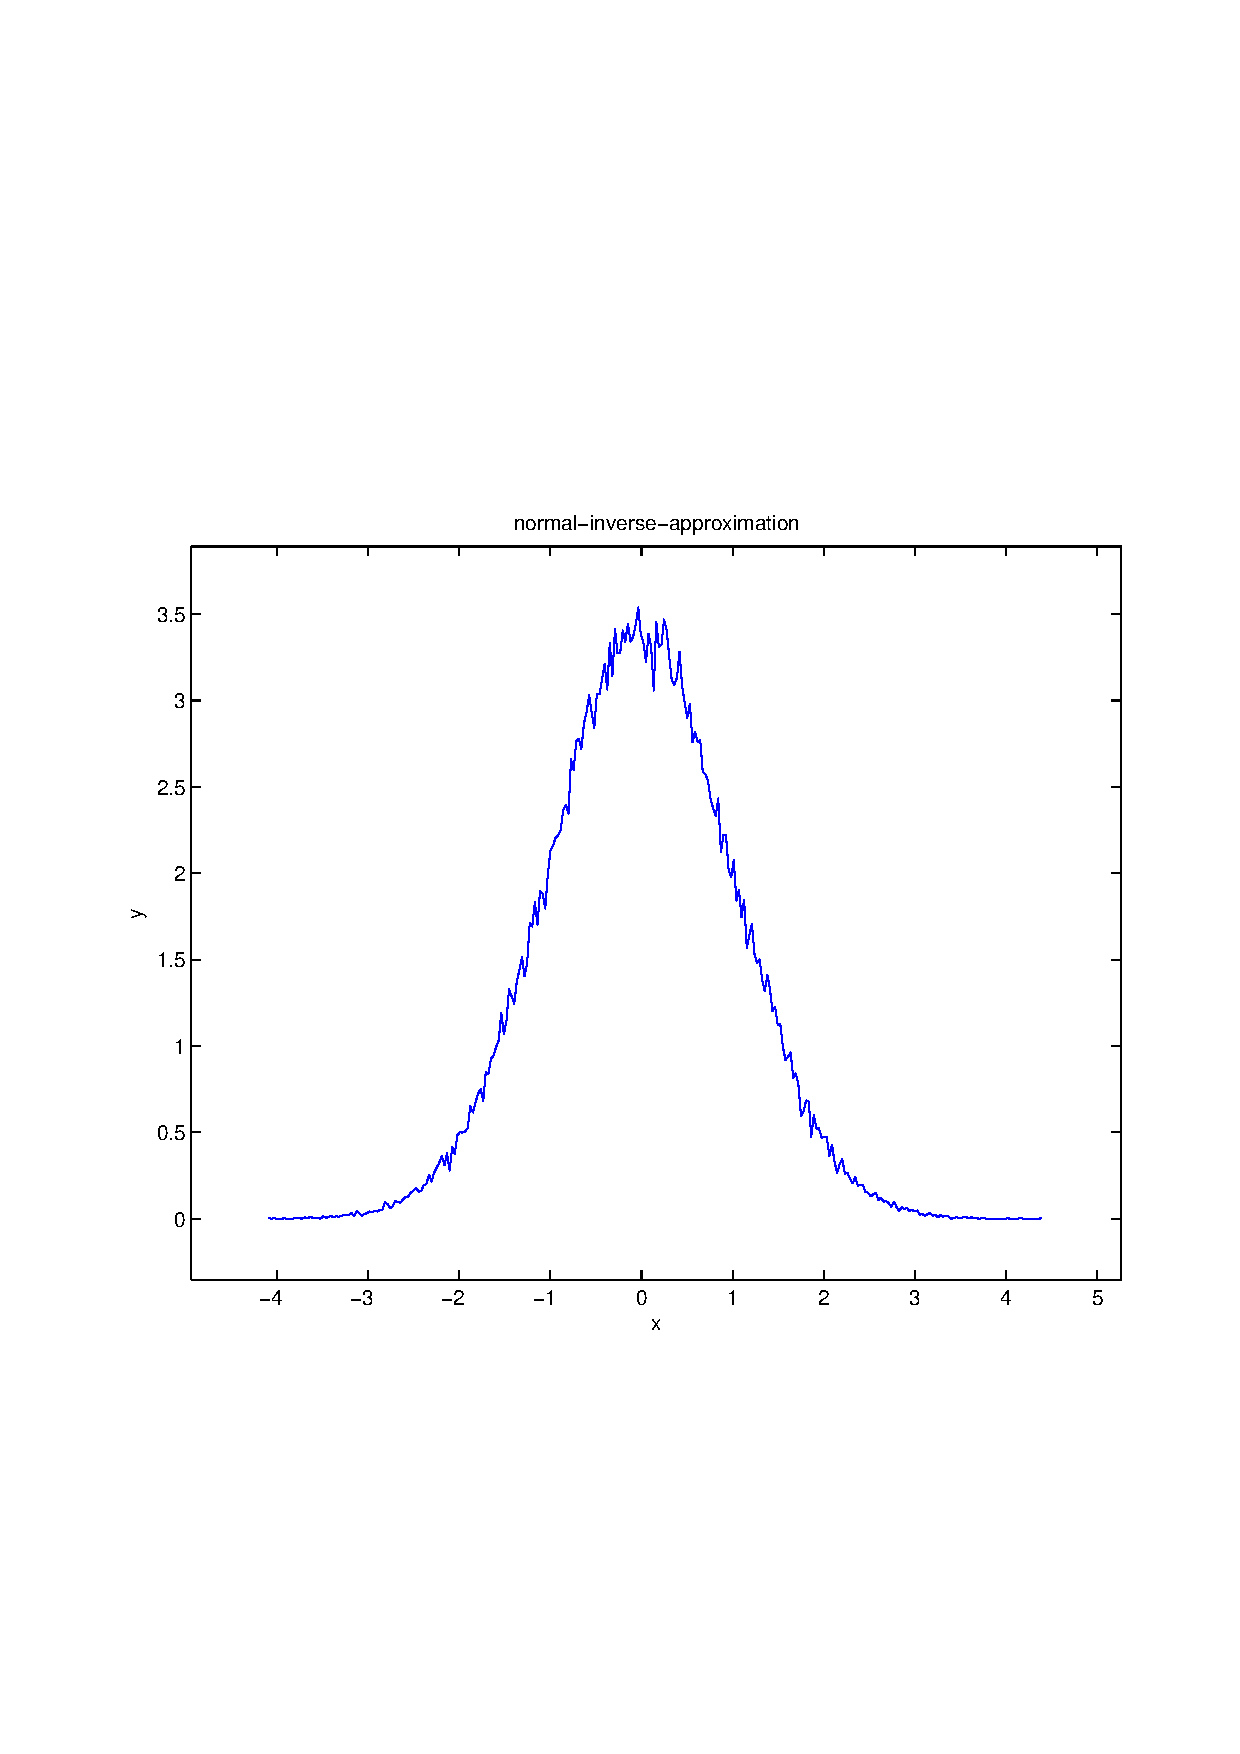
\includegraphics[width=5cm,height=5cm]{normal-inverse-approximation.pdf}

pareto \begin{tabular}{|c|c|c|c|}  mean & variance & skewness & kurtosis \\  \hline
$\mu_1 = +3184578.265$ & $\mu_2 = +888468246174112900.000$ & $\mu_3 = +315.370$ & $\mu_4 =+99629.098$ \\
\end{tabular}

\includegraphics[width=5cm,height=5cm]{pareto.pdf}

poisson \begin{tabular}{|c|c|c|c|}  mean & variance & skewness & kurtosis \\  \hline
$\mu_1 = +1.107$ & $\mu_2 = +0.133$ & $\mu_3 = +3.854$ & $\mu_4 =+20.137$ \\
\end{tabular}

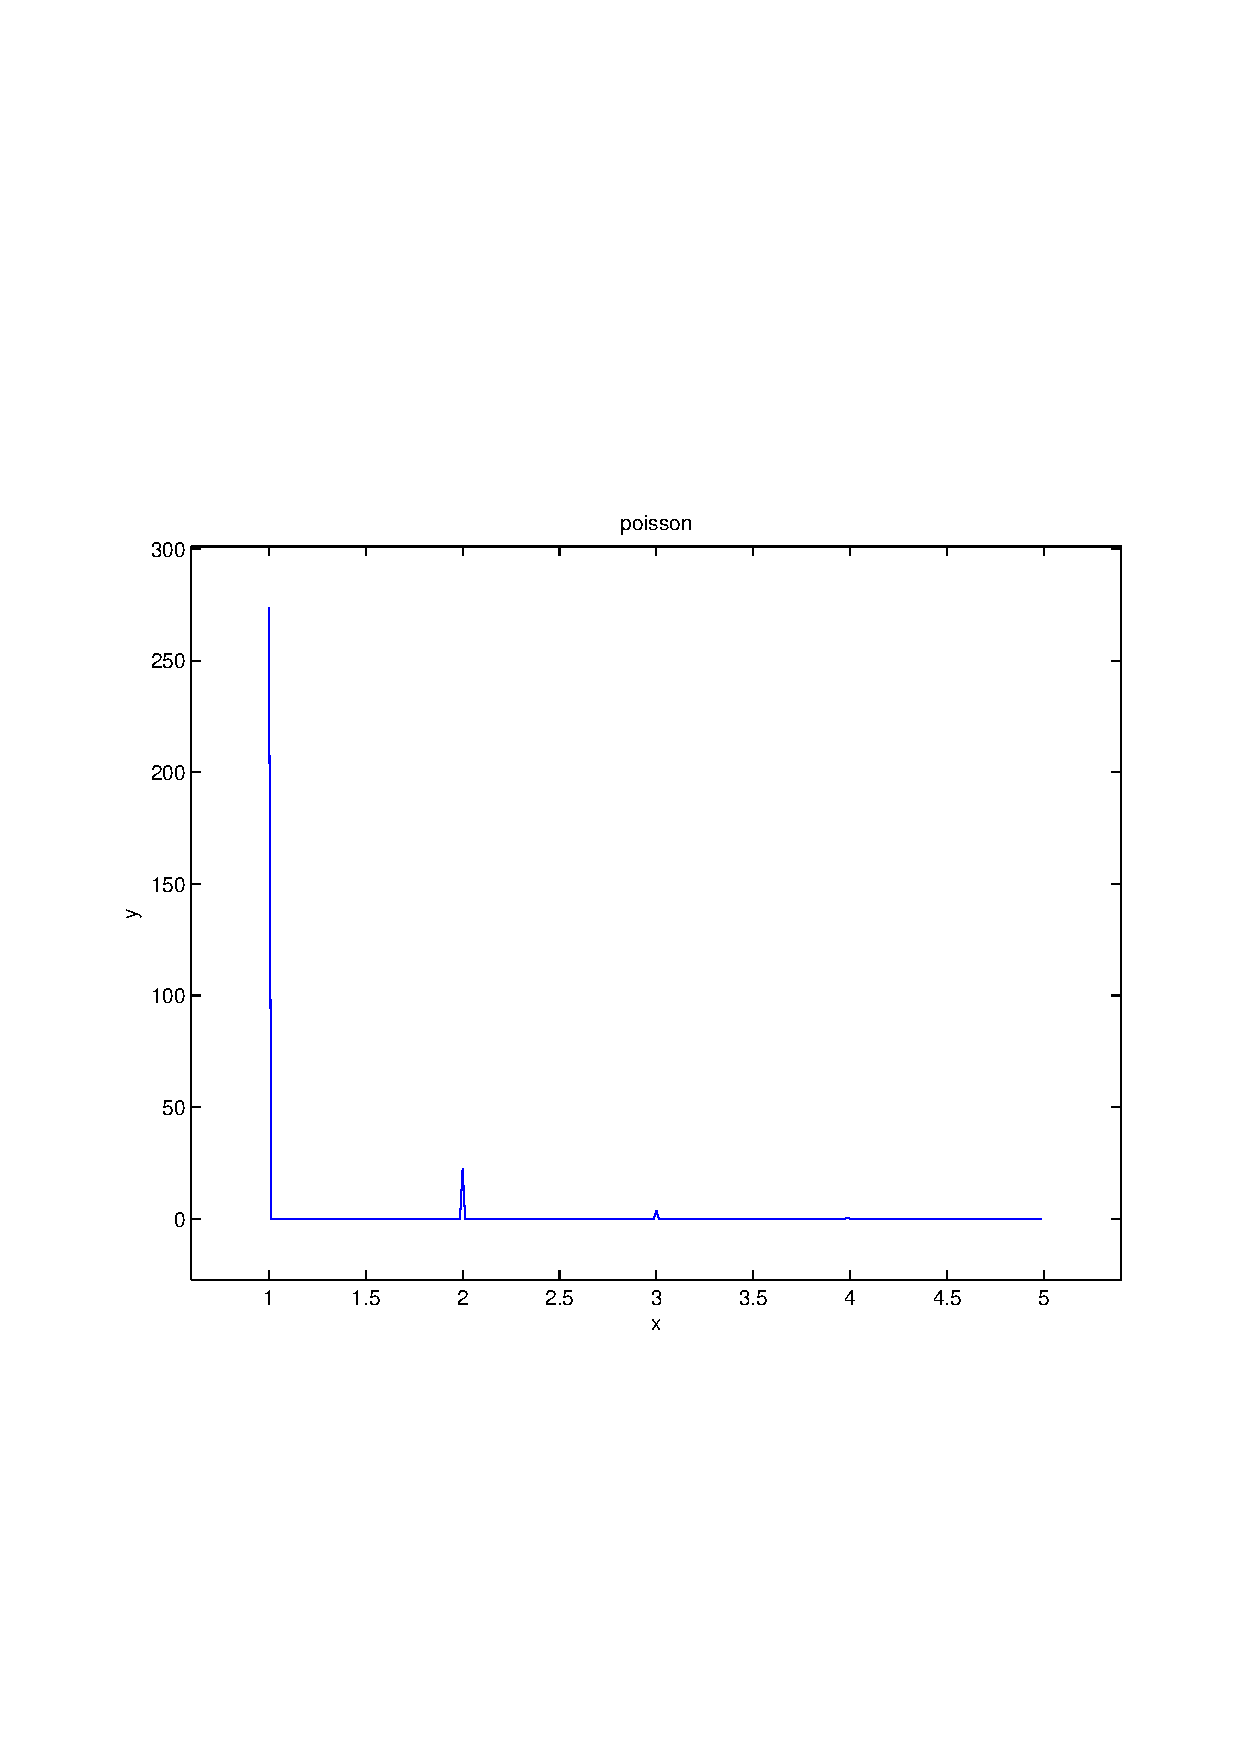
\includegraphics[width=5cm,height=5cm]{poisson.pdf}

\newpage
beta \begin{tabular}{|c|c|c|c|}  mean & variance & skewness & kurtosis \\  \hline
$\mu_1 = +0.334$ & $\mu_2 = +0.127$ & $\mu_3 = +0.678$ & $\mu_4 =+1.904$ \\
\end{tabular}

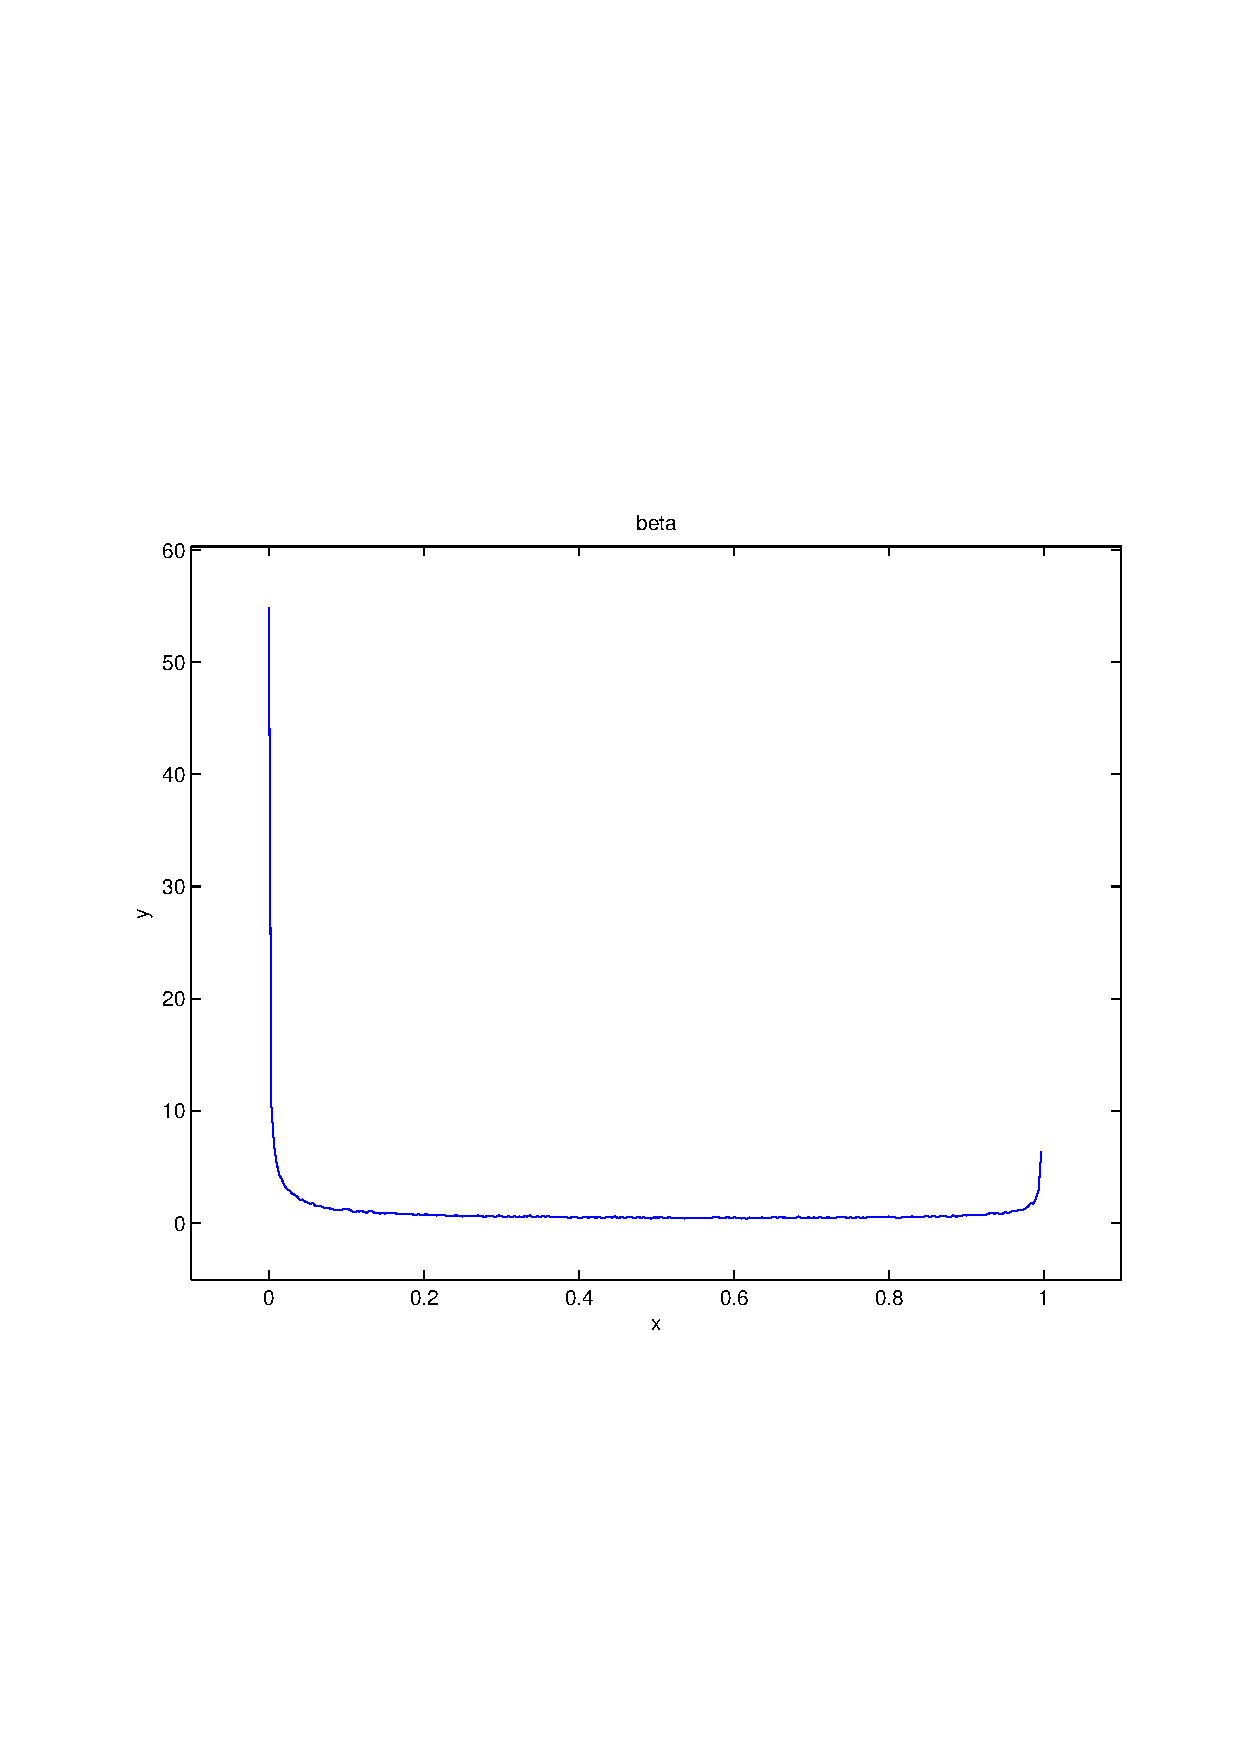
\includegraphics[width=5cm,height=5cm]{beta.pdf}

QueryPerformanceCounter  =  +20.372
\subsubsection{ARPACK}
Running Arnoldi Krylov algorithm on an $n=64$ dimensional $GOE$ matrix.
\subsubsection{Semidefinite Programming SDPA}
QueryPerformanceCounter  =  +0.048
\subsubsection{Linear Regression 3x1}
\subsubsection{3 x 1 Linear Regression}
Sample size = 64

Number of features = 3

$\sigma = \left(
\begin{array}{
ccc}
+3.952 & -0.499 & -0.010 \\
-0.499 & +1.895 & +0.465 \\
-0.010 & +0.465 & +4.477 \\
\end{array}
\right)$

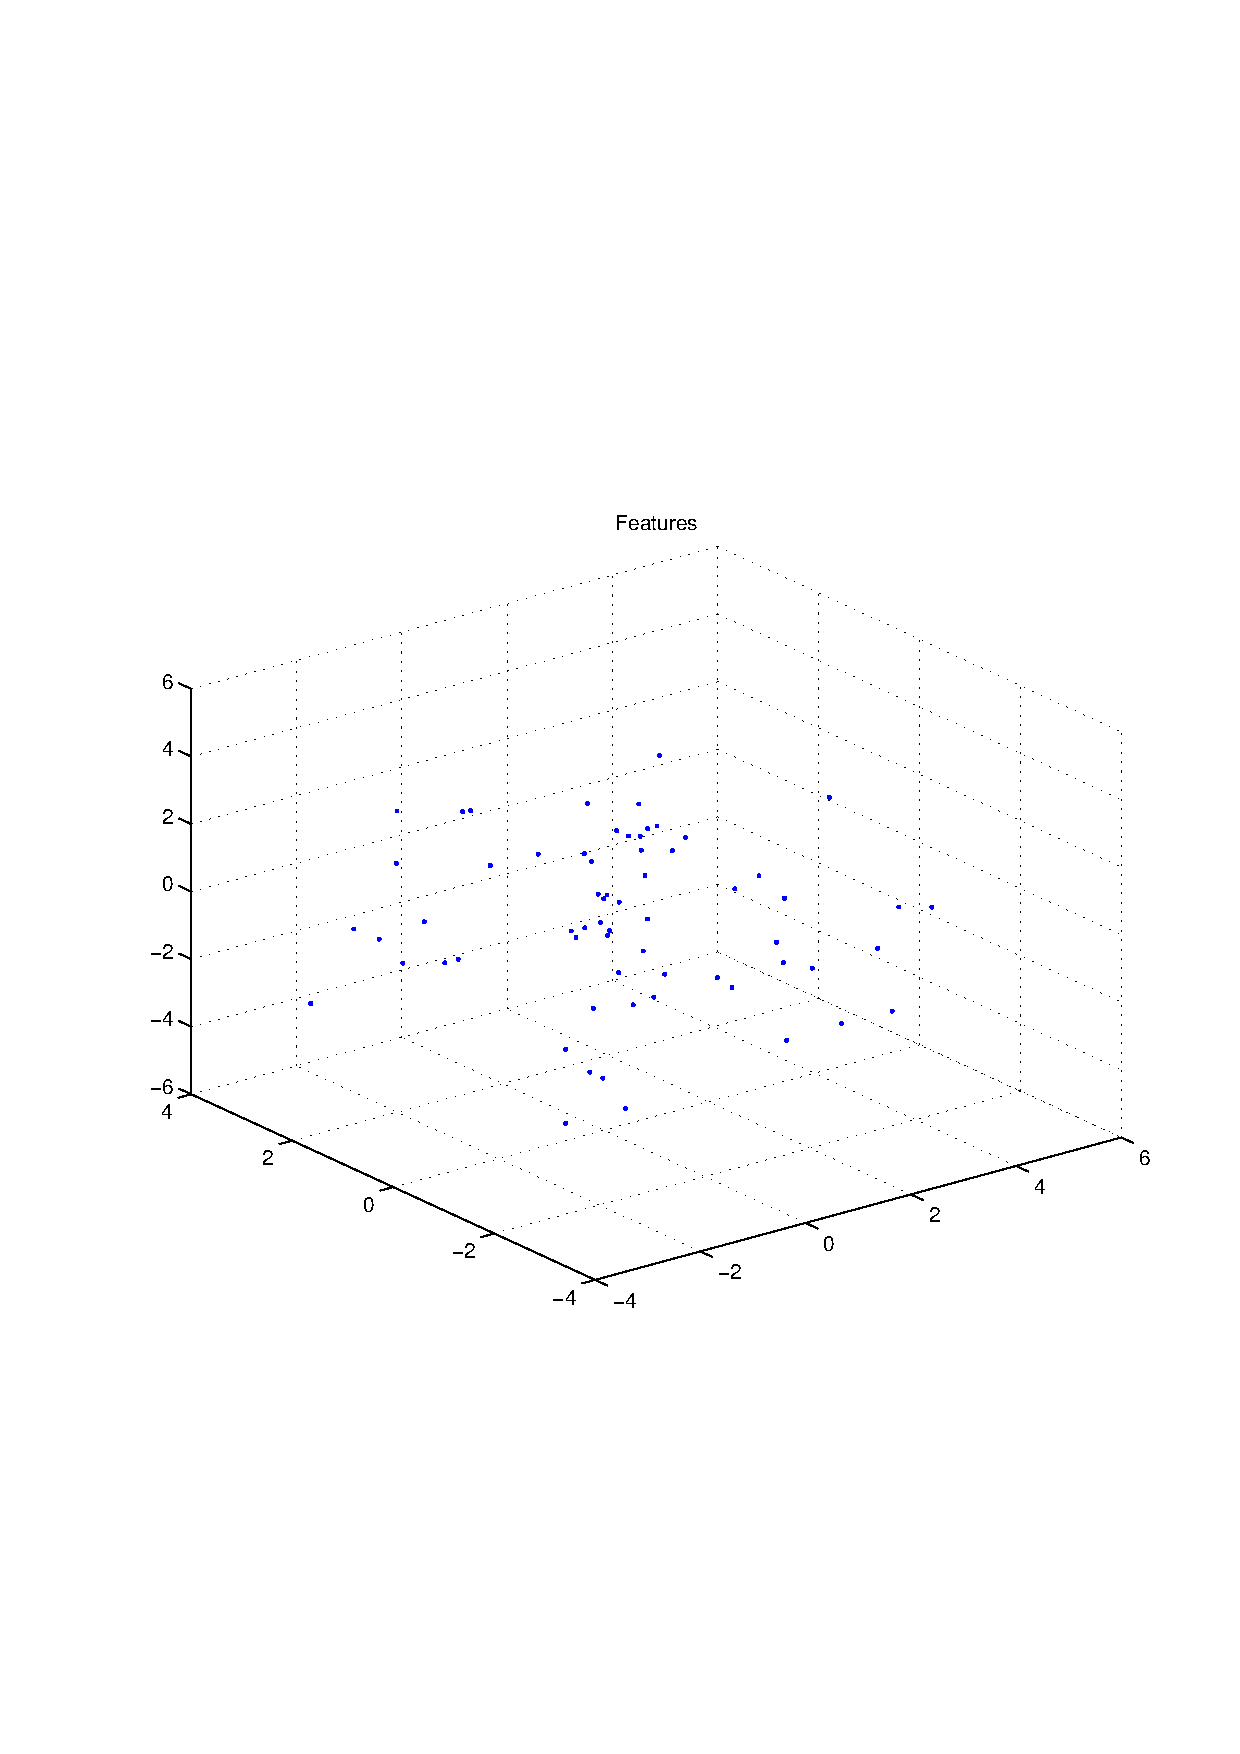
\includegraphics[width=10.0cm,height=10.0cm]{regression_features.pdf}

Beta
+0.817, +0.999, +0.510

Response
-1.556
+1.646
+0.823
+1.951
-1.180
+2.637
+1.032
+2.236
+1.501
+3.123
+6.030
+2.843
-0.264
+2.594
-1.496
+4.679
-1.284
+3.382
-0.002
+0.292
-2.349
+1.969
-0.883
+1.741
-2.196
+0.167
+1.954
-0.382
+2.594
+1.768
+0.206
+2.527
+3.786
+0.641
-2.539
+3.293
+2.862
+1.013
-4.378
+0.767
+1.151
+1.372
-0.731
+0.541
-1.676
+0.773
-2.951
+1.592
-0.036
+0.711
-2.029
+0.987
+0.894
-5.999
+0.609
-2.656
+3.157
-2.163
-1.809
+0.595
-3.867
-0.003
+0.802
+3.602
Estimate for Beta
-6277438562204192200000000000000000000000000000000000000000000000000.000
-6277438562204192200000000000000000000000000000000000000000000000000.000
-6277438562204192200000000000000000000000000000000000000000000000000.000
Error:
-0.000, +0.000, -0.000


QueryPerformanceCounter  =  +1.079
\subsubsection{Matrix Norms}
\subsubsection{Haar Distributed Random Orthogonal Matrix $A \in O(n)$}
 Testing Operator Norm
Number of Dimensions: 3435973836

\subsubsection{Generate Tracey Widom Sample}
\subsubsection{Sample from $W_n m$ times and calculate empirical PDF of the first eig}
This test of the KL libraries will generate histograms of 		  $\lambda_1$ for GOE (Gaussian Orthogonal Ensemble), and W (Wishart) 		  distribution of random matrices

This should approximate the celebrated Tracy Widom distribution.
Dimension $n = 1024$

Sample size $m = 2048$

